% don't remove the following lines, and edit the definition of \main if needed
\documentclass[../report.tex]{subfiles}
%\usepackage[utf8]{inputenc}
\providecommand{\main}{..}
\IfEq{\jobname}{\currfilebase}{\AtEndDocument{\biblio}}{}
% until here


%defined commends for flow section
\providecommand*{\psin}{\ensuremath{\Psi_{n}}}
\providecommand*{\ppb}{\ensuremath{p}+Pb}
\providecommand*{\pbpb}{Pb+Pb}
\providecommand*{\pt}{\ensuremath{p_{\mathrm{T}}}}



\begin{document}

\section{Flow and Correlations}

\textbf{Coordinators}: Soumya Mohapatra (Columbia University)

\linebreak

\textbf{Contributors}: Alexandru Florin Dobrin (CERN), Stefan Floerchinger (University of Heidelberg), Wei Li (Rice University), Vitaly Orokov (National Research Nuclear University MEPhI), Bjoern Schenke (Brookhaven National Lab)



\subsection{Introduction}

High energy nuclear collisions at RHIC and the LHC produce a relativistic fluid composed of QCD matter, i. e. quarks and gluons. It is particularly interesting to study the macroscopic properties of this fluid because - at least conceptually - they are fully fixed by the microscopic properties of a renormalizable, fundamental quantum field theory, namely QCD. One can study here experimentally, as well as theoretically, how macroscopic material properties result from microscopic field theoretic processes. Many theoretical methods ranging from perturbative to non-perturbative techniques are being developed to understand this in detail and one can expect that the insights gained here will be valuable for many related problems in fields ranging from condensed matter theory to cosmology in the future.  

One must say that currently the field is still largely driven by experimental progress. Theoretically, the connection between microscopic QCD physics and the macroscopic properties of the quark-gluon plasma are being understood step by step but a satisfactory understanding is still missing. 

Many different fronts of research are being explored at the moment. This ranges from conceptual questions on how to consistently formulate relativistic fluid dynamics or how to solve quantum field theory in non-equilibrium situations to very concrete practical questions about the thermodynamic and transport properties (such as viscosities or conductivities) of the quark-gluon plasma. Besides the role of strong interactions, also electromagnetic interactions and in particular the role of magnetic fields and the production of photons and dileptons is being explored. Other fronts of research concern the role of quantum anomalies, chirality and vorticity or the dependence of collective behavior on system size (nucleus-nucleus versus proton-nucleus and proton-proton collisions), on centrality and collision energy, the initial state directly after the collision, or various types of fluctuations. We will discuss these issues in more detail in the following subsections.


\begin{itemize}
	\item General introduction
	\item Why is it interesting to study the fluid dynamics of the QGP
	\item What has been learnt so far at LHC 
	\item What questions remain
\end{itemize}
 %Bjoren,Stefan +(Soumya)
\clearpage
\subsection{Identified particle \vn}\label{sec:identified_particle_vn}


\begin{figure}[!htb]
\begin{center}
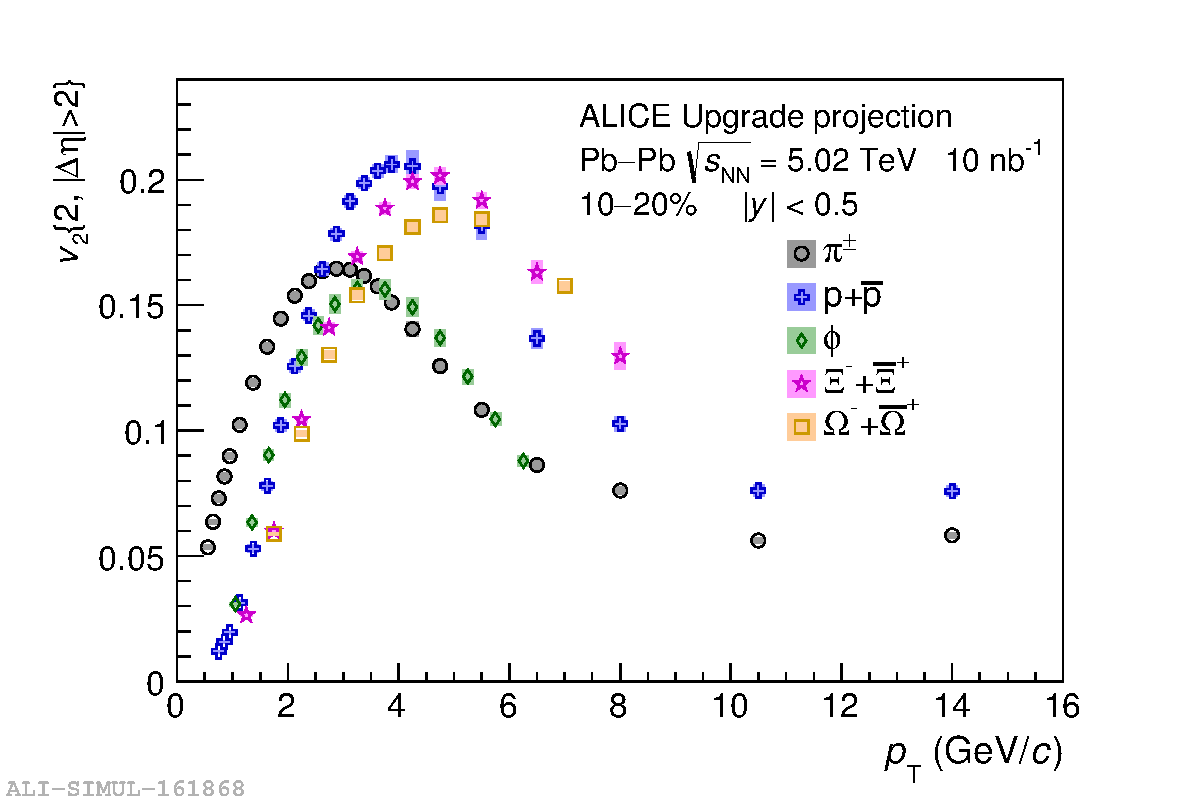
\includegraphics[width=0.495\textwidth]{\main/flow/figs/alice_projection_pid_v2}
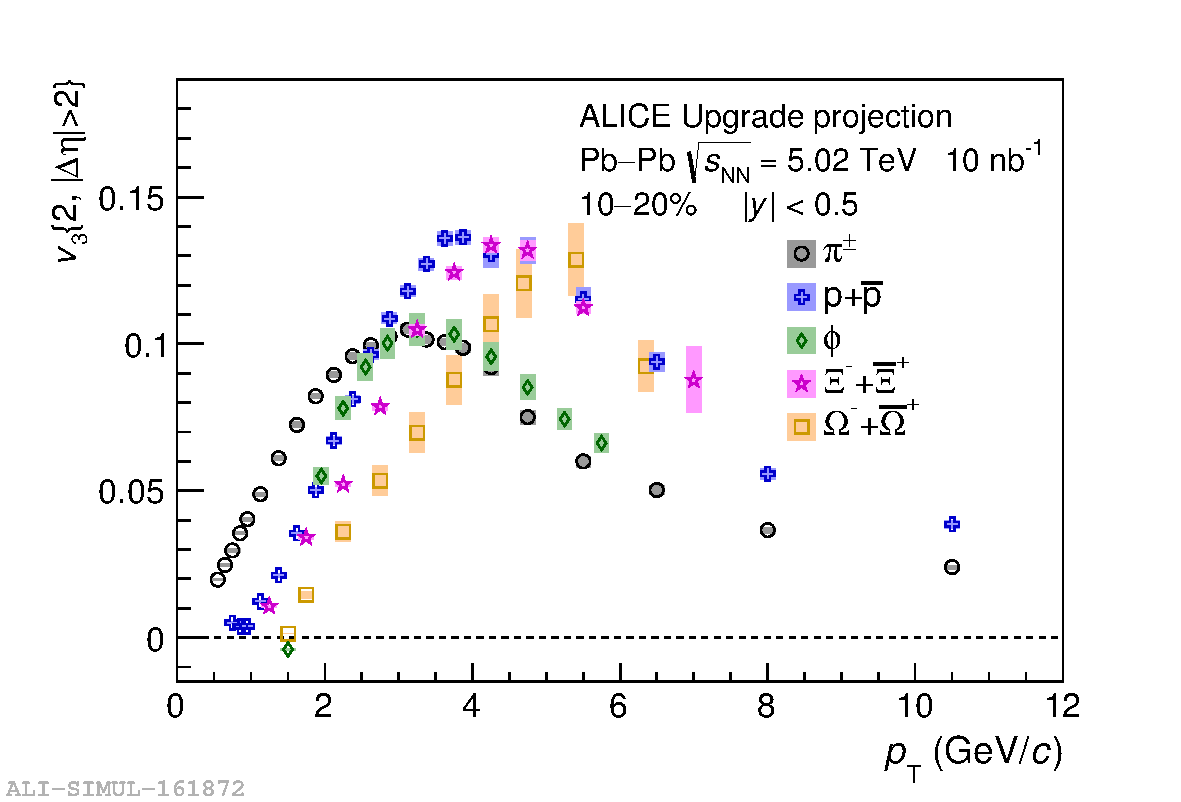
\includegraphics[width=0.495\textwidth]{\main/flow/figs/alice_projection_pid_v3}
\caption{
ALICE projections for $v_2$ (left) and $v_3$ (right) of $\pi^\pm$, 
  $\mathrm{p}$+$\overline{\mathrm{p}}$, $\Xi$+$\overline{\Xi}$, 
  $\Omega$+$\overline{\Omega}$, and the $\phi$-meson 
  in the 10--20\% centrality interval
  for an integrated luminosity of 10~nb$^{-1}$. 
Error bars (shaded boxes) represent the projected statistical 
  (systematic) uncertainties.}
\label{fig:alice_vn}
\end{center}
\end{figure}

As stated earlier most \vn\ measurements for inclusive hadrons are the LHC 
  are not statistics limited.
However for identified particles there is considerable scope for reduction 
  in statistical uncertainties in Run~3 and 4.
This is true both for heavy-flavor particles 
  as well for identified light flavour hadrons.
Figure~\ref{fig:alice_vn} shows projections from the ALICE collaboration for 
  the $v_2$ and $v_3$ of several light-flavor species, that are expected for 
  an integrated luminosity of 10~nb$^{-1}$ expected in Run~3 and 4.
The projected statistical uncertainties are typically negligible over the 
  entire \pt\ range and in most cases the systematic uncertainties are 
  quite small as well.

As stated before, the increased precision of these measurements will help in 
  better understanding of the QGP equation of state. 
These measurements will also lead to an improved understanding 
  of the hadronization mechanism at the QGP$\rightarrow$hadron transition.
Additionally, detailed measurements of constituent quark scaling (or its violation)
  can provide constraints on the contribution of the subsequent hadronic 
	rescattering, into the final azimuthal anisotropy of the final particles.
This is because the azimuthal anisotropy developed in the QGP phase 
  (as a function of transverse energy) is expected to scale with the 
	number of constituent quarks, while the anisotropy developed in the hadronic
	phase is different depending on the particle species.


\begin{figure}[!htb]
\begin{center}
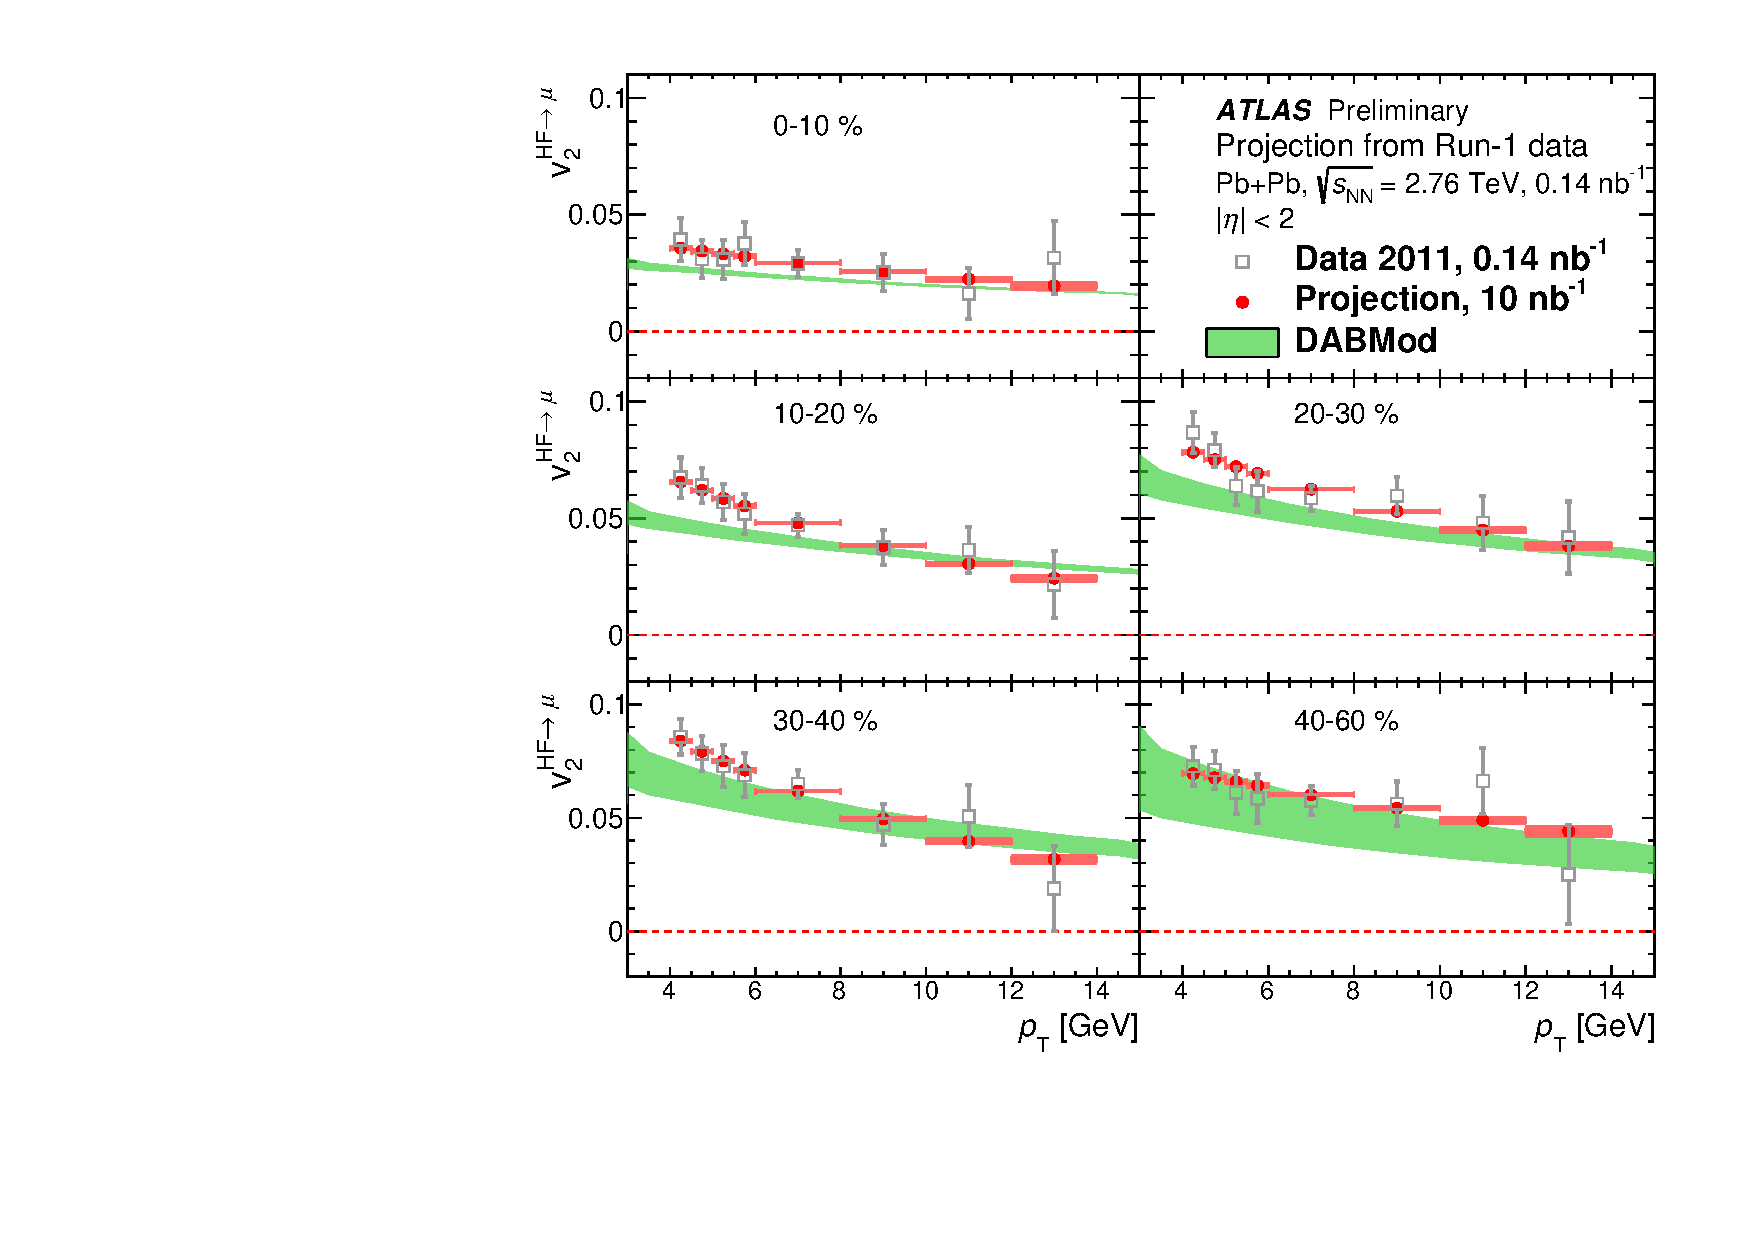
\includegraphics[width=1.0\textwidth]{\main/flow/figs/atlas_hfmuonv2}
\caption{
ATLAS projections of $v_2$ as a function of \pt, for muons from the decay of 
  heavy-flavor hadrons. 
Each panel corresponds to a different centrality interval. 
The present measurements are also shown for comparison. 
The error bars (shaded boxes) correspond to statistical uncertainties only. 
The projections are also compared to calculations from the DABMod model.}
\label{fig:atlas_hf_v2}
\end{center}
\end{figure}

Figure~\ref{fig:atlas_hf_v2} shows projections from the ATLAS collaboration
  for the $v_2$ of muons produced from the decay of heavy-flavor hadrons
  in Run~3 and 4, showing a considerable improvement in the statitical 
  precision of the measurement.
The central values of the projections are obtained by fitting the 
  present measurements with an exponential function, which qualitatively 
  describes the present data. 
The statistical uncertainties in the projections are made by scaling down 
  the present uncertainties to correspond to the expected luminosity in 
  Run~3 and 4 (10~nb$^{-1}$).
Calculations from the DABMod model~\cite{Prado:2016szr} are also shown,
  which demonstrate the inability of the present measurements
  in establishing or ruling out models due to limited statistical precision.
The flow measurements for heavy quarks is important as they are produced at
  earlier times in the heavy-ion collision and thus are susceptible
  to the full time evolution of the QGP.
The heavy-flavor anisotropy measurements can determine if heavy-quarks couple 
  strongly or weakly to the QGP, and additionally can constrain the heavy-quark 
  transport and diffusion coefficients.
Chapter~\ref{sec:HI_HF} has further discussions of Run~3 and 4 flow projections
  for heavy-flavor particles and their physics implications. 


%\subsection{QCD Equation of State}
%The QCD equation of state, accessible in high-energy collisions (and in the region around mid-rapidity) is that at vanishing baryon chemical potential, and it has been established for some time that it features a crossover transition to a chirally symmetric quark gluon plasma \cite{Aoki:2006we}. Most recent lattice calculations \cite{Steinbrecher:2018phh} have determined the cross-over temperature to be $T_c\simeq 156.5 \pm 1.5\,{\rm MeV}$. Recent efforts are also exploring the equation of state at finite $\mu_B$, which at LHC would have relevance mainly at very forward rapidities. Here, because of the sign problem, methods like Taylor expansion \cite{Kaczmarek:2011zz,Endrodi:2011gv,Bazavov:2015zja,Bonati:2018nut} or imaginary chemical potentials \cite{Cea:2014xva,Bonati:2014kpa,Bonati:2015bha,Bellwied:2015rza,Cea:2015cya} have to be employed. 

%To employ lattice QCD based equations of state in hydrodynamic caluclations, they need to be matched to a hadron resonance gas model at low temperatures, to cover the entire temperature range from zero to the maximally reached teperature. Various equations of state \cite{Huovinen:2009yb, Borsanyi:2013bia, Bazavov:2014pvz}, using different lattice data and different matching conditions have been used in simulations. A comparison of some of them can be found in \cite{Moreland:2015dvc}. In this work the sensitivity of observables to the choice of equation of state was studied. While the mean transverse momentum varied by approximately 3\% when using different equations of state, $v_2$ and $v_3$ changed by 8\% and 15\%, respectively. Because different lattice data was used, and matching to the hadron resonance gas was performed at a higher temperature, the s95p-v1 lattice parameterization has a smaller speed of sound in an extended temperature regime, compared to the other equations of state. This leads to a reduced amount of flow. 

%Such differences will affect the precise extraction of transport coefficients, such as $\eta/s$ and $\zeta/s$. Fortunately, the newer lattice QCD equations of state from the hotQCD collaboration \cite{Bazavov:2014pvz} and the Wuppertal-Budapest collaboration \cite{Borsanyi:2013bia} lead to differences only on the percent level for the studied observables.

%Currently, the experimental data can not easily teach us directly about the equation of state, because of the uncertainty in the transport coefficients. One possibility would be to extend state of the art Bayesian techniques \cite{Moreland:2018gsh} to include free parameters describing the equation of state and fit them along with other free parameters such as shear and bulk viscosities. 

%\subsection{Shear viscosity of hot nuclear matter}
%Ideal fluid dynamics has been very succesful in describing a variety of bulk observables in heavy ion collisions \cite{Kolb:2003dz,Huovinen:2003fa,Hirano:2002ds}, indicating early on that the shear and bulk viscosities of the produced matter cannot be large. Calculations in the strong coupling limit using gauge gravity duality have found a value of $\eta/s=1/4\pi$ for an $N = 4$ super Yang-Mills quantum system. This value was significantly smaller than the $\eta/s$ obtained in perturbative QCD calculations, which were, however, plagued by significant errors, mainly resulting from uncertainties in the relevant scales \cite{Arnold:2003zc}. Recently, such perturbative calculations have been extended to include next-to-leading order corrections and aa significant reduction compared to the leading order result was found \cite{Ghiglieri:2018dgf}: At temperatures of the order of the QCD transition the NLO $\eta/s$ is smaller by a factor of $5$ compared to the LO result, and reaches values of approximately $2/4\pi$. 

%Extractions of transport coefficients from lattice QCD calculations \cite{Nakamura:2004sy,Meyer:2007ic,Pasztor:2018yae} are extraordinarily hard, because the spectral function for use in the Kubo formula follows from a difficult inversion of an integral transform of a correlator of the energy momentum tensor. Most recent calcaultations for a pure gluon plasma find $\eta/s=0.17\pm 0.02$ at $T=1.5\,T_c$.

%Apart from above direct calculations of the shear viscosity to entropy density ratio, by means of hydrodynamic simulations its value can be extracted by comparison to experimental data \cite{Gale:2013da,Heinz:2013th}. This method suffers mainly from uncertainties in the initial state (see Section \ref{sec:initialstate}). The latest constraints come from simulations using the IP-Glasma initial state \cite{Schenke:2012wb,Schenke:2012fw}, the EKRT model \cite{Niemi:2015qia} and Bayesian analyses employing the Trento initial state model \cite{Moreland:2018gsh}. IP-Glasma + hydrodynamic simulations including bulk and shear viscosity find for the shear viscosity an effective constant value of $\eta/s=0.095$ at the $\sqrt{s}=2.76\,{\rm TeV}$ LHC energy and $\eta/s=0.06$ at the top RHIC energy. EKRT simulations find good agreement with LHC data using a constant value of $\eta/s=0.2$ and also certain temperature dependent $\eta/s$ values. Finally, the latest Bayesian analyses of $\sqrt{s}=5\,{\rm TeV}$ Pb+Pb collisions at the LHC using the Trento initial state determined an approximately linearly rising $\eta/s$ with temperature, with $(\eta/s)(T=150\,{\rm MeV})\approx 0.09$ and $(\eta/s)(T=300\,{\rm MeV})\approx 0.16$.

%The method of extracting $\eta/s$ using hydrodynamic simulations and comparison to experimental data thus leaves us with an uncertainty of approximately a factor of $3$ at this point. Comparison to more observables that would allow to independently better constrain features of the initial state and medium properties will hopefully reduce this uncertainty in the future. 


%\subsection{Bulk viscosity of hot nuclear matter}
%There are several theoretical indications that bulk viscosity could play an important role in the transition region of QCD (see \cite{Ryu:2017qzn} and references therein). Similar to the case of shear viscosity, bulk viscosity over entropy density ratios have been calculated using holography in the strong coupling regime using extensions to non-conformal theories \cite{Buchel:2007mf,Finazzo:2014cna}. The temperature dependent $\zeta/s$ features a peak of value 0.05 around a temperature of $\sim 160\,{\rm MeV}$. 
%Perturbative calculations have shown that the simple estimate $\zeta\approx 15 \eta(1/3-c_s^2)^2$ \cite{Horsley:1985dz} is parametrically correct for QCD \cite{Arnold:2006fz}, where $(1/3-c_s^2)$ is the deviation from conformal symmetry. Lattice calculations using the Kubo formula extract large values of $\zeta/s$ around $T_c$ \cite{Karsch:2007jc,Meyer:2007dy}, with large uncertainties for the value at $T_c$, which is of order 1 \cite{Kharzeev:2007wb}, and exhibit a fast drop with increasing $T$.

%Parametrizations of the bulk viscosity over entropy density's temperature dependence were performed in \cite{Denicol:2009am} with input from \cite{Karsch:2007jc} for the QGP phase and \cite{NoronhaHostler:2008ju} for the hadronic phase. This parametrization features a peak of $\zeta/s$ around $T\approx 180\,{\rm MeV}$, reaching approximately a value of 0.3. It has been used in various hydrodynamic simulations employing the IP-Glasma initial state and led to good agreement of the calculated mean transverse momentum with experimental data. Calculations using other initial states have reported the need for smaller bulk viscosity over entropy density values. For example in a recent Bayesian analyss using the Trento initial state model, $\zeta/s$ peaks at a value about 10 times smaller. In \cite{Schenke:2018fci} it was discussed how the compact size and initial flow present in the IP-Glasma initial state contribute to the need for a larger bulk viscosity compared to other initial state models. 

%Viscous corrections to the distribution function at freeze-out affect the low $p_T$ part of the spectrum more for bulk viscosity than for the shear part \cite{Bozek:2009dw,Paquet:2015lta}. Consequently, the uncertainties resulting from bulk viscous corrections are typically larger than for shear when studying $p_T$ integrated observables. 

%\subsection{Heat conductivity}
%Bulk diffusion, can we constrain it?

%\subsection{Electric conductivity}
%can we constrain it? Relevance for magnetic fields, Chiral magnetic effect
%
% Bulk diffusion and electric conductivity are now being discussed in the section on light flavors. (Stefan F.)
%


%\subsection{Second order transport properties}
%A peculiar feature of relativistic fluid dynamics is that it is not always causal. More specifically,  this problem arises when one goes beyond the ideal fluid approximation and includes dissipative transport properties such as shear viscosity,  bulk viscosity and heat conductivity or baryon diffusion. Keeping for the shear stress,  bulk viscous pressure and baryon diffusion current only terms of first order in gradients of the fluid velocity,  temperature and chemical potential leads to a covariant version of the well known Navier-Stokes theory,  which however,  is not an hyperbolic differential equation and can therefore not be used for a time evolution that is causal in the relativistic sense. A way out has been proposed by Müller,  as well as Israel and Stewart. In their framework,  the theoretical setup is modified in such a way that the shear stress,  bulk viscous pressure and baryon diffusion current are not related to the gradients of fluid velocity and thermodynamic variables by constraints but rather have their own evolution equation and relax towards the Navier-Stokes values on a proper time scale given by their respective relaxation times. These relaxation times cannot be too small in order to have a causal set of fluid dynamic evolution equations.

%It would in fact be great to test the modifications proposed by Müller,  Israel and Stewart (and subsequent authors) experimentally and to put an experimental bound on the value of the relaxation times (or their ratios to other thermodynamic and transport properties). This would help for a better understanding of relativistic fluid dynamics that is also needed elsewhere,  for example in cosmology. However,  this is not very easy and can only be done in an interplay of theory and experiment. In fluid dynamic models of heavy ion collisions one can vary the value of second order transport coefficients and study the impact on various flow observables,  in particular particle spectra,  flow coefficients $v_n$,  flow correlation functions and HBT parameters. By a detailed comparison to experimental data one can put constraints on the second order transport coefficients. It might become possible to vary second order transport coefficients in global Bayesian analysis calculations and provide experimental constraints in this way. A large variety of experimental flow observables,  detailed and differential data,  as well as small statistical uncertainties are obviously helpful for this endeavor.


%Bjoern, Stefan, Soumya
\clearpage


\section{Initial conditions} \label{sec:initialstate}
As already alluded to in Section \ref{sec:macro}, the intial state of heavy ion collisions is the major source of uncertainty when it comes to extracting transport properties of the produced medium. This has to do with the fact that calculations of the exact geometry and its fluctuations involve nonperturbative physics. The available descriptions for the initial state thus range from very simplistic models that assign deposited energy densities based on the wounded nucleons or binary collisions determined in a Monte-Carlo Glauber prescription, to classical effective theories of QCD that are valid in the high energy limit. The latter are certainly closer to first principles calculations, and should provide a realistic description of the initial state assuming that the high energy limit is a good approximation.

The major ingredient that needs to be provided by an initial state model is the geometry of the interaction region in the plane transverse to the beam. It is entirely dominated by the positions of incoming nucleons whose fluctuations also play an important role. Observables are also sensitive to the detailed way the energy is deposited given a distribution of wounded nucleons, and the constraints on this from data are surprisingly robust \cite{Moreland:2018gsh}. Using the Trento model it was found that the product of thickness functions of the two nuclei at every given transverse position gives the best description of the data (compared to a conventinal wounded nucleon model or other combinations of thickness functions). This type of energy deposition is very much what the EKRT \cite{Niemi:2015qia} and IP-Glasma \cite{Schenke:2012wb,Schenke:2012fw} models include, explaining their success in describing a wide range of observables \cite{Niemi:2015qia,Gale:2012rq}.

Fluctuations of wounded nucleon positions contribute the dominant effect to fluctuations of the initial geometry in heavy ion collisions. Smaller scale fluctuations (emerging e.g. from color charge fluctuations in the IP-Glasma model) have been shown to not significantly affect most observables measuring the momentum anoisotropy of produced particles \cite{Gardim:2017ruc}. The factorization breaking ratio shows some sensitivity and it should be pointed out that multiplicity fluctuations are also influenced by the existence of color charge fluctuations.

More recently, indications that the nucleon should possess a substructure of hotspots have emerged. The IP-Glasma model was unable to describe flow coefficients in p+Pb collisions assuming a round proton \cite{Schenke:2014zha}. Including subnucleonic fluctuations constrained by incoherent diffractive $J/\psi$ production data from HERA \cite{Mantysaari:2016ykx} (which also require a fluctuating proton geometry) improved the agreement with the p+Pb data significantly \cite{Mantysaari:2017cni}. Recent Bayesian analyses also found that nucleon substructure is necessary to simultaneously describe p+Pb and Pb+Pb bulk observables \cite{Moreland:2018gsh}.
It should be noted, however, that the size scales for nucleons and subnuclear hot spots extracted in that work are significantly larger than those obtained from comparison to HERA data in the IP-Glasma model.

Initial conditions for hydrodynamic simulations have to provide, in principle, all components of the energy momentum tensor as a function of spatial position (and initial conditions for other conserved charges, if considered). This includes, apart from the always included energy density distribution, the initial flow as well as initial viscous corrections. Initial flow is included in many recently developed models, that either assume free streaming \cite{Moreland:2018gsh}, including Yang-Mills evolution, which is close to free streaming \cite{Gale:2012rq} or an initial flow distribution motivated by strong coupling calculations \cite{Weller:2017tsr}. Initial viscous corrections are often set to zero. Only a few works \cite{Mantysaari:2017cni,Schenke:2018fci,Moreland:2018gsh} include the full viscous stress tensor provided by the initial state description.

Since the initial state models that provide the entire $T^{\mu\nu}$ all switch from essentially a freely streming system to strongly interacting hydrodynamics at a fixed time $\tau$, that transition is somewhat abrupt and not very physical. To improve over this situation an intermediate step using effective kinetic theory has been introduced \cite{Kurkela:2018wud,Kurkela:2018vqr}. This procedure allows for a somewhat smoother matching but has yet to be used in full fledged hydrodynamic simulations. The effect on observables in heavy ion collisions is likely small, while in small systems, such as p+A a larger effect can be expected.

As already discussed in Section \ref{sec:macro}, the choice of initial state has a significant effect on the extraction of transport coefficients. A more compact initial state and the presence of initial flow lead to a larger transverse flow, which requires a larger bulk viscosity to compensate for it and produce agreement with experimental data \cite{Schenke:2018fci}. Also, the models' eccentricities will affect the final momentum anisotropies, influencing the extracted shear viscosity to entropy density ratio. Two possible attempts to solve this problem have been pursued: Constrain an initial state description as well as possible using data from experiments other than heavy ion collisions (e.g. e+p scattering data, which will hopefully be extended to e+A in a future electron ion collider facility), or perform a combined Bayesian analysis of all parameters, including those of the initial state, to find the best fit for all transport coefficients along with the initial state description.

As mentioned above, at the moment the two approaches lead to some similar features of the initial state (product of thickness functions, presence of subnucleon structure), but also show discrepancies (size of the nucleon and sub-nucleon scales along with the size of the extracted bulk viscosity). Only when the two methods converge for all features of the initial state and medium properties, can one confidently declare that the initial state as well as the transport properties of the QGP are understood.
\clearpage
%\subsection{Fluctuations of conserved charges} 
\label{sec:fluctuations}
\subsubsection{Physics introduction and observables}

In the phase diagram of strongly interacting matter at zero net baryon density, the presence of a chiral phase transition between hadronic matter and a QGP has been conjectured \cite{Pisarski:1983ms}, and arguments have been presented~\cite{Ejiri:2009ac,Ding:2018auz} in lQCD that the transition, for vanishing light quark masses, is of second order and belongs to the O(4) universality class. Due to the small but finite physical quark masses, in lQCD a rapid crossover is found \cite{Aoki:2006we,Aoki:2009sc,Borsanyi:2010bp,Bazavov:2011nk,Bhattacharya:2014ara} which, however, exhibits pseudo-critical features due to the smallness of the u- and d-quark masses and the proximity of the crossover region to the O(4) line \cite{Ejiri:2009ac,Ding:2013lfa}. 

In general, fluctuations can be linked to critical behaviour associated with a phase transition, and it has been pointed out that fluctuations of conserved charges in heavy-ion collisions can provide an experimental observable to test for critical behaviour in the phase diagram of strongly interacting matter \cite{Ejiri:2005wq,Bazavov:2017dus,Friman:2011pf,Bazavov:2012jq}. These fluctuations can be related to susceptibilities, specifically to the derivatives of the pressure with respect to the chemical potentials corresponding to the conserved charges. Here, the relevant `charges' are baryon number $B$, strangeness $S$, and electrical charge $Q$, and the corresponding chemical potentials are $\mu_B$, $\mu_S$, and $\mu_Q$. The susceptibilities are defined (see e.g. \cite{Bazavov:2012jq,Bellwied:2015lba}) in terms of dimensionless normalized chemical potentials \(\hat{\mu}_X\equiv \mu_X/T \) \: as

\begin{equation}
\chi_{ijk}^{BQS}(T) = \left.
\frac{\partial P(T,\hat{\mu})/T^4}{\partial\hat{\mu}_B^i \partial\hat{\mu}_Q^j \partial\hat{\mu}_S^k}\right|_{\hat{\mu}=0} \; .
\label{suscept}
\end{equation} 

\noindent The generalized susceptibilities can be computed in lQCD at vanishing chemical potential, exactly the conditions probed by experiments at the LHC. Within the Grand Canonical Ensemble (GCE), these generalized susceptibilities can be related to experimental measurements of the fluctuations of particle multiplicities, such as the net number of baryons. For instance, a measurement of higher moments or cumulants of net baryon number in relativistic nuclear collisions can be directly related \cite{Karsch:2010ck,Skokov:2012ds,Karsch:2012wm,Karsch:2017mvg,Borsanyi:2013hza,Borsanyi:2014ewa} to theoretical predictions from lQCD or from more phenomenological models of the chiral phase transition \cite{Almasi:2017bhq,Parotto:2018pwx} to shed light on the possible critical behaviour near the QCD phase boundary. 
For a distribution of the net baryon number, $\Delta N_B = N_B - N_{\overline{B}}$, with moments defined as 

\begin{equation}
\mu_i = \langle (\Delta N_B - \langle \Delta N_B \rangle )^i \rangle ,
\end{equation}
the cumulants $\kappa_i$ can be directly linked to the generalized susceptibilities such as

\begin{equation}
\kappa_2 = \mu_2 = VT^3 \chi_2^B
\end{equation}
\begin{equation}
\kappa_3 = \mu_3 = VT^3 \chi_3^B  
\end{equation}
\begin{equation}
\kappa_4 = \mu_4 - 3\mu_2^2 = VT^3 \chi_4^B.
\end{equation}


\begin{figure}[ht]
\begin{center}
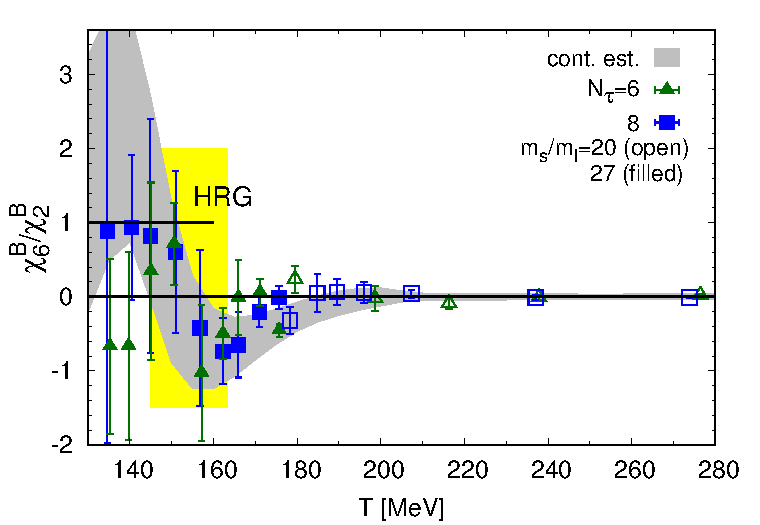
\includegraphics[width=0.45\textwidth]{\main/lightflavour/figs/B6_B2_wideT_27.pdf}
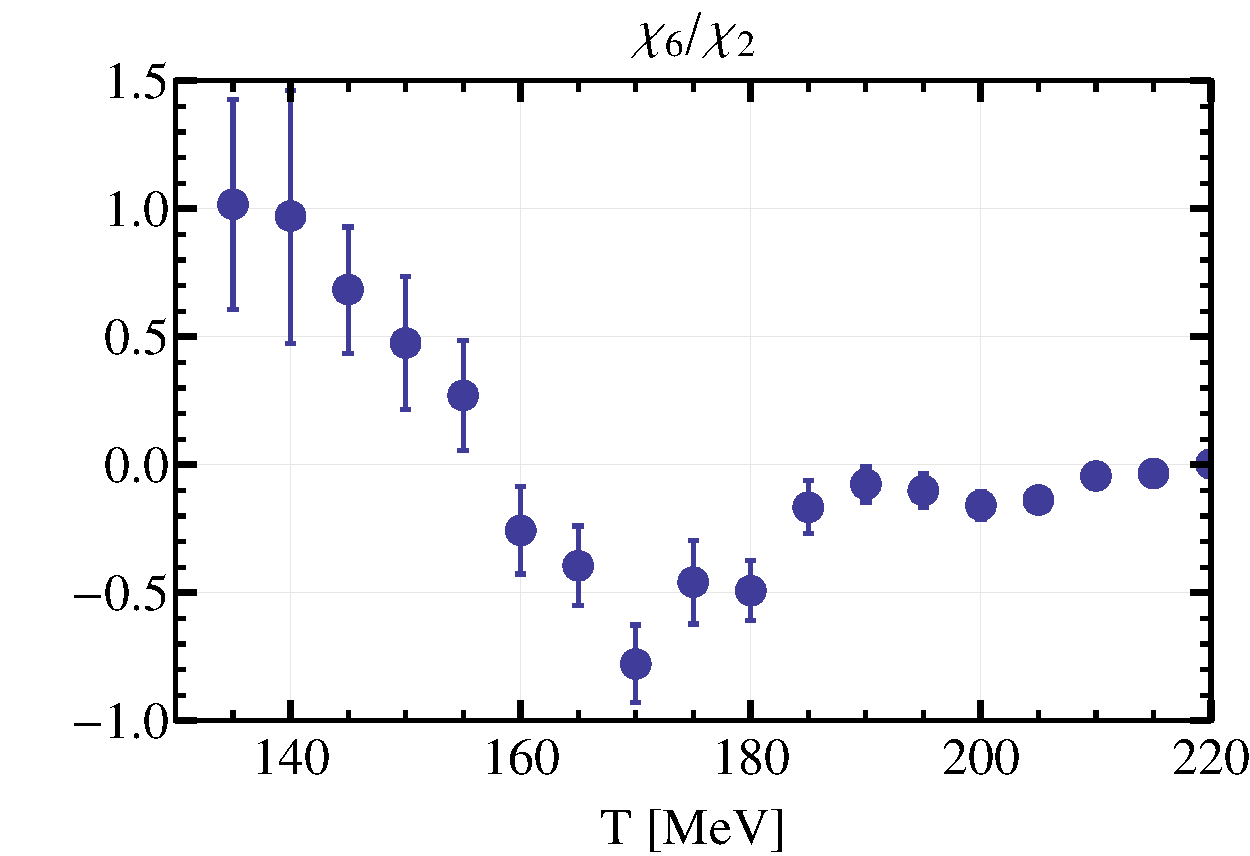
\includegraphics[width=0.46\textwidth]{\main/lightflavour/figs/c6c2_fromLattice.pdf}
\end{center}
\caption{Ratio of sixth to second-order baryon number susceptibilities from lQCD. The left-hand figure is from \cite{Bazavov:2017dus}. The right-hand figure is calculated from recent lQCD data on  sixth and  second  order susceptibilities from \cite{Borsanyi:2018grb}. }  
\label{fig:chi62}
\end{figure}

In the O(4) universality class, a singular contribution to the pressure shows up for higher order  moments.
More specifically, at vanishing chemical potential, all odd susceptibilities of the net baryon number vanish.  
In addition, in the O(4) universality class, the second- and fourth-order susceptibilities remain finite  at  the  phase  transition  temperature  at $\mu_B~=~0$  in  the  chiral  limit,
implying  that  only  sixth-  and  higher-order  susceptibilities  diverge \cite{Ejiri:2005wq,Friman:2011pf}. Thus, for  physical  quark  masses and at $\mu_B~=~0$, only higher order cumulants $\kappa_n$ with $n\geq 6$ can exhibit O(4) criticality,  whereas at finite $\mu_B$ this is already the case for $\kappa_n$ with $n\geq 3$.  

Sensitivity to chiral criticality due to the vicinity of the O(4) line at $\mu_B~=~0$ is borne out in phenomenological models as is shown in \cite{Friman:2011pf,Almasi:2017bhq}, and in lQCD predictions \cite{Bazavov:2017dus,Borsanyi:2018grb}, by strong deviations of $\chi_6^B/\chi_2^B$ from unity as shown in Fig.~\ref{fig:chi62}.

We note that a convenient baseline for the cumulants of multiplicity distributions and fluctuations of produced particles in relativistic nuclear collisions can be obtained in the framework of the hadron re\-so\-nance gas (HRG) \cite{Allton:2005gk,Karsch:2010ck,BraunMunzinger:2011ta,Borsanyi:2018grb,Luo:2017faz}. In this model, uncorrelated Poissonian fluctuations of baryon and anti-baryon multiplicities result in a Skellam distribution for the net baryon number, in which the higher moments and cumulants can all be related to the first moments in the following way \cite{BraunMunzinger:2011ta,BraunMunzinger:2011dn, Braun-Munzinger:2018yru}:
\begin{equation}
\label{lbaseline}
\kappa_n(N_B - N_{\overline{B}}) = \langle (N_B +(-1)^n N_{\overline{B}}) \rangle
\end{equation}
For zero net baryon number then all odd cumulants vanish and all even cumulants are identical.

Measuring such cumulants with precision poses a formidable experimental challenge due to the requirement of very large data sets ($> 10^9$ events of a particular event or centrality class) with superb control of systematic uncertainties. As a first physics case to consider along this line, the impact of measuring the distribution of net protons as a proxy for net baryons needs to be studied further. We note that, at LHC energy and low transverse momentum, particle production near mid-rapidity takes place mostly in gluonic processes, implying that isospin asymmetries, as in the colliding nuclei, are absent. As a consequence, the production yields of protons and neutrons should be very close. For light nuclei this isospin symmetry has been checked experimentally, albeit with significant uncertainties. 
In addition, non-critical contributions to the cumulants from volume fluctuations and global baryon number conservation \cite{Skokov:2012ds,Braun-Munzinger:2016yjz, Braun-Munzinger:2018yru} need to be evaluated and the data corrected accordingly. Furthermore, in particular for comparison to lQCD predictions, care needs to be taken to keep experimental cuts such as in \pT\ to a minimum insofar as such cuts cannot be introduced in lQCD \cite{Karsch:2015zna,Alba:2015iva}.
     
Two-particle correlations with net baryons can also be used to explore transport properties of the hydrodynamic evolution. The baryon diffusion constant $D$ is a fundamental transport property of the quark-gluon plasma, similar to shear viscosity $\eta$ or bulk viscosity $\zeta$. It characterizes the mobility of baryon number, and is predicted to be finite at the LHC despite the fact that $\mu_{B}\sim0$. A two-particle correlation function as been proposed~\cite{Floerchinger:2015efa}, which explores correlations of net-baryon fluctuations as a function of separations in azimuthal angle and rapidity, and can provide experimental constraints on the diffusion coefficient $D$. As $\mu_{B}\sim0$ at the LHC, such an analysis has yet to be carried out in Run 1 and 2 data since it is statistically challenging, and will be greatly aided by the increase by about a factor 100 in the \PbPb integrated luminosity foreseen for Runs 3 and 4.

\subsubsection{State of the art experimental measurements and present limitations}

Net proton fluctuations measured by the ALICE experiment and in the STAR beam energy scan program provide interesting and stimulating results. The measurements at STAR~\cite{Adamczyk:2013dal} complement the corresponding measurements from ALICE, which will make it possible to pin down the global structure of the phase diagram of strongly interacting matter in a wide range of temperatures and net-baryon densities. However, before drawing firm conclusions by confronting theoretical calculations with  data, non-dynamical contributions stemming from unavoidable fluctuations of  participant nucleons and  overall baryon number conservation have to be subtracted from the experimental measurements. Both of these non-dynamical contributions, which exist neither in lQCD nor in the HRG model, lead to deviations from the baseline as defined in Eq.~\ref{lbaseline}. Indeed, the acceptance dependence of the second-order cumulants of net-protons measured by ALICE~\cite{Rustamov:2017lio} exhibits deviations from the non-critical (Skellam) baseline. However, these deviations were explained by global baryon number conservation~\cite{Rustamov:2017lio, Braun-Munzinger:2016yjz, Braun-Munzinger:2018yru}, which, in accordance with the experimental findings, decreases the amount of fluctuations with the increasing acceptance. This is the first experimental verification of the lQCD predictions for the second-order cumulants of net-baryon distributions. This also serves as a strong support of the HRG model, in that experimental measurements of the second cumulants of net-protons do not show any evidence of criticality and actually coincide with the second cumulants of the Skellam distribution.  In order to probe critical phenomena, higher cumulants beyond the second order have to be addressed. 

As mentioned in the previous section, even at vanishing net-baryon densities, lQCD and other theoretical calculations such as Polyakov-loop extended Quark- Meson model (PQM)~\cite{Almasi:2017bhq} predict critical fluctuations encoded in the deviations of net-baryon $\kappa_{4}/\kappa_{2}$ and $\kappa_{6}/\kappa_{2}$ from unity. Moreover, at the pseudo critical temperature of about 156 MeV the magnitudes of $\kappa_{4}/\kappa_{2}$ and $\kappa_{6}/\kappa_{2}$  are predicted in Ref.~\cite{Almasi:2017bhq} to be 0.5 and -0.39, respectively. Similar values of $\kappa_{6}/\kappa_{2}$ are quoted in different lQCD calculations as presented in Fig~\ref{fig:chi62}.  These numbers, shown in  Fig.~\ref{netpALICE_STAR}, do not take into account experimental artefacts such as global net-baryon number conservation and unavoidable fluctuations of participating nucleons from event to event. Also shown are the values of of $\kappa_{4}/\kappa_{2}$ and $\kappa_{6}/\kappa_{2}$ after accounting for these non-dynamical effects using the procedure in Refs.~\cite{Braun-Munzinger:2016yjz, Braun-Munzinger:2018yru}. Even after accounting for participant fluctuations and global baryon number conservation we observe deviations in $\kappa_{4}/\kappa_{2}$ and $\kappa_{6}/\kappa_{2}$ from unity, although they are somewhat reduced.   This motivates our experimental program  of measuring higher moments of net-proton distributions at the LHC energies. Also, fluctuation measurements  are underway in the strange baryon sector to approach measurements of net baryon number fluctuations. All this will be greatly helped by the anticipated dramatic increase in statistics in Runs 3 and 4.

\begin{figure}[ht]
\begin{center}
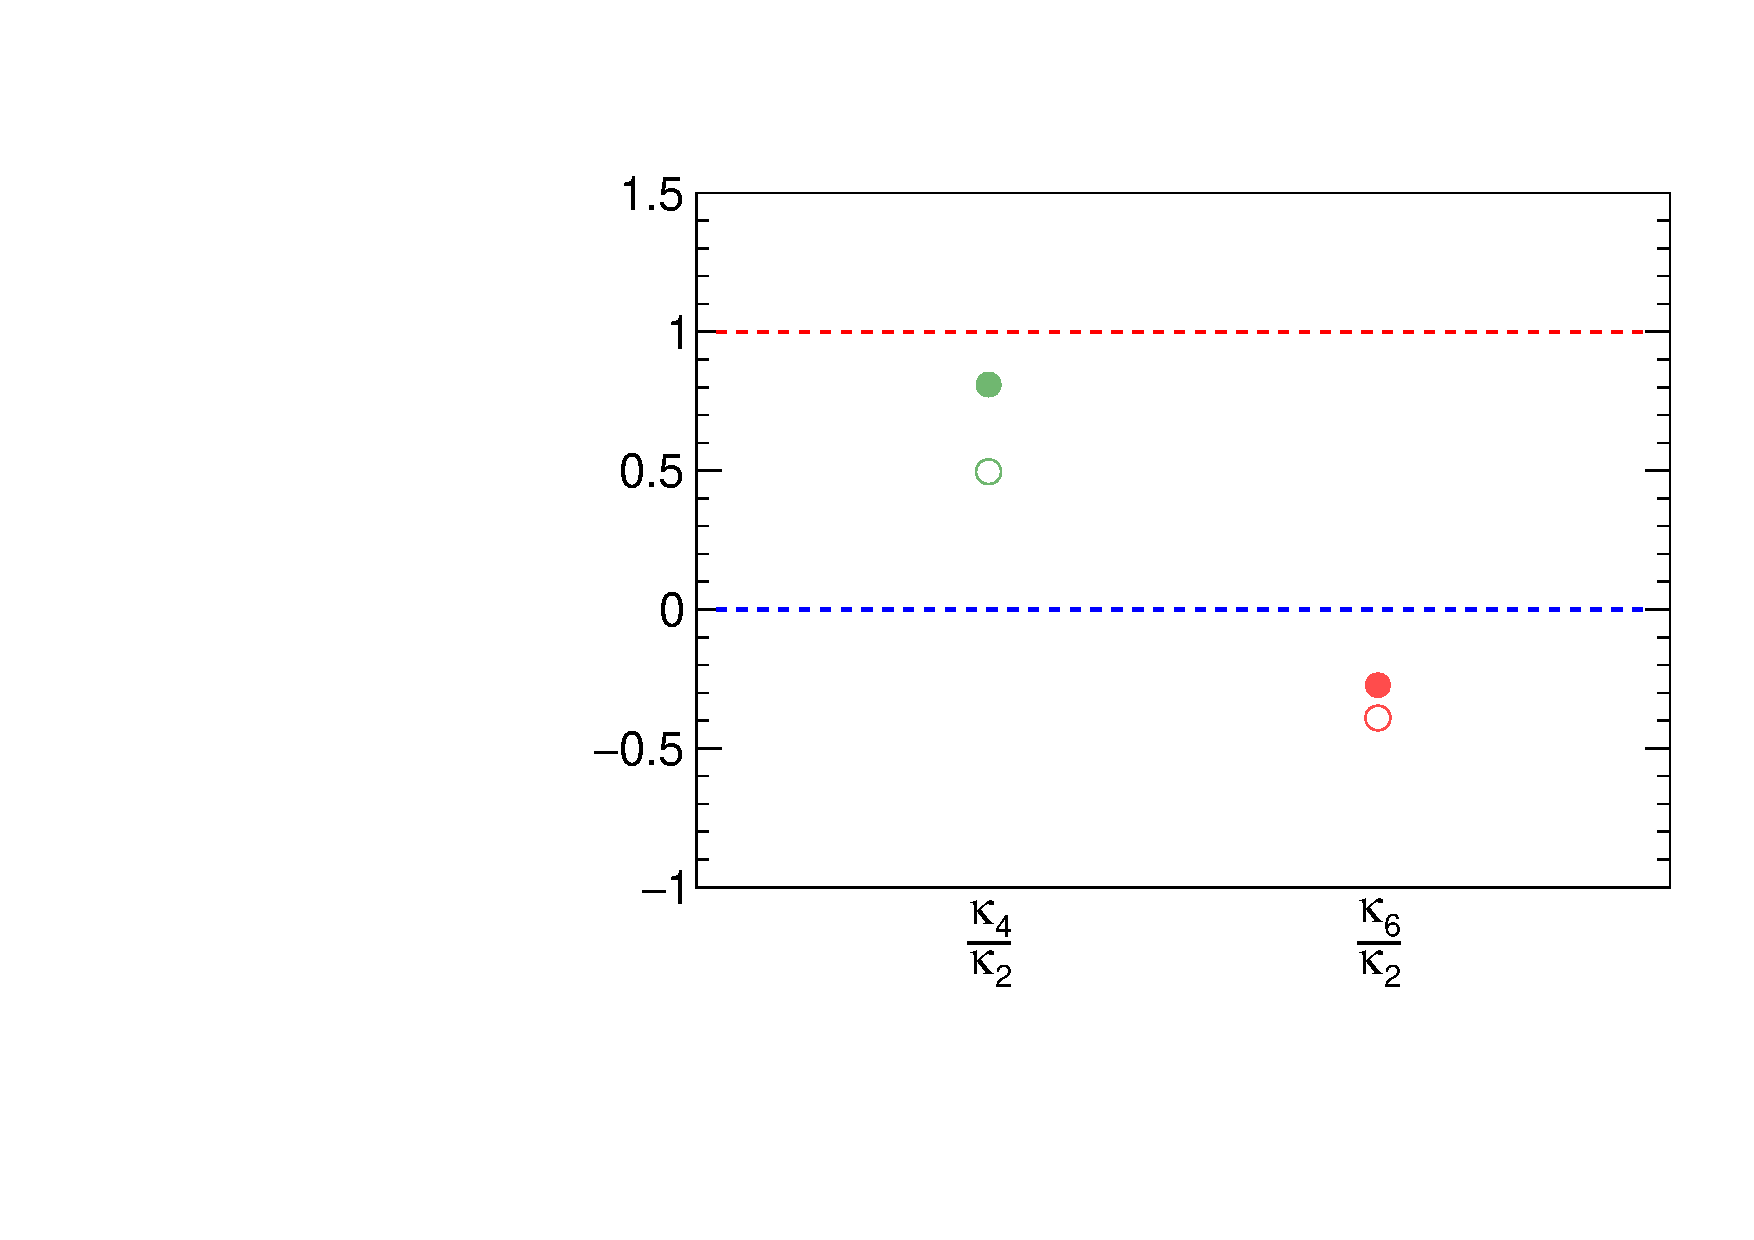
\includegraphics[width=0.6\textwidth]{\main/lightflavour/figs/baseLine.pdf}
\end{center}
\caption{$\kappa_{4}/\kappa_{2}$ and $\kappa_{6}/\kappa_{2}$  as calculated within PQM~\cite{Almasi:2017bhq} model (open symbols).  After taking into account contributions from participant nucleon fluctuations and global baryon number conservation~\cite{Braun-Munzinger:2016yjz, Braun-Munzinger:2018yru}, the deviations from unity decrease (closed symbols).} 
\label{netpALICE_STAR}
\end{figure}

\subsubsection{Projections for HL-LHC}

As discussed above, precise studies of the higher-order cumulants of particle multiplicity distributions are needed to verify theoretical predictions. In this section we estimate the statistics needed to address these measurements with the ALICE experiment. For this purpose two distinct  Monte Carlo simulations have been developed. In the first approach, following recent developments in~\cite{Bzdak:2018axe}, the probability distribution function of net-protons is approximated  by a superposition of two Gaussian distributions which has four free parameters. Using the experimentally measured second cumulant of net-protons for 0-5 \% most central \PbPb collisions~\cite{Rustamov:2017lio} and the $\kappa_{4}/\kappa_{2}$ and $\kappa_{6}/\kappa_{2}$ ratios from the PQM model~\cite{Almasi:2017bhq}, we first obtained absolute values for $\kappa_{4}$ and $\kappa_{6}$.  These values were adjusted to account for fluctuations from participant nucleons in 0-5$\%$ most central \PbPb collisions and global baryon number conservation~\cite{Braun-Munzinger:2016yjz, Braun-Munzinger:2018yru}. Finally, the free parameters of the double Gaussian distribution were fixed using the expected values of $\kappa_{1}$ , $\kappa_{2}$ , $\kappa_{4}$ and $\kappa_{6}$ , where $\kappa_{1}$ equals zero by definition. The event-by-event net-proton number was sampled from the double Gaussian function  thus generating the net-proton distribution for a given number of events. 
In the second approach the probability distribution functions of protons and anti-protons are calculated separately by exploiting the Pearson curve method \cite{Behera:2017xwg}. This approach also needs four measurements as inputs, which are taken as the first four cumulants of the proton and anti-proton multiplicities measured by ALICE (presented in \cite{Behera:2018wqk}).  The net-proton distribution for a given number of events is constructed by sampling the obtained proton and anti-proton probability distribution functions. 
In each approach, the resulting statistical uncertainties are obtained using the subsample method.  

The obtained results for $\kappa_{4}/\kappa_{2}$ and $\kappa_{6}/\kappa_{2}$ and their corresponding statistical uncertainties are shown in Fig.~\ref{fig:c4c2toymc} as a function of the simulated event statistics. The dashed red lines correspond to the input values predicted by PQM calculations of critical fluctuations (CF) and assuming a double Gaussian net-proton distribution, while the green dashed lines come from the Pearson curve method based on the lower-order cumulants measured by ALICE. As expected, with increasing statistics both $\kappa_{4}/\kappa_{2}$ and $\kappa_{6}/\kappa_{2}$ approach their nominal values. The statistics necessary to measure these cumulants are presented in the bottom panels of Fig.~\ref{fig:c4c2toymc}, where the deviations of the expected values from unity are quantified in terms of the magnitudes of the statistical uncertainty ($\sigma$). As seen from the left panel of Fig.~\ref{fig:c4c2toymc}, for $\kappa_{4}/\kappa_{2}$ already 10 million events are sufficient to distinguish the expected critical fluctuations signal from  unity with a statistical significance of $4\sigma$. Similar conclusions are obtained with the Pearson curve method.  Several times this amount of data has already been recorded by ALICE, and the expected statistics in Run 3 and Run 4 will make it possible to measure  $\kappa_{4}/\kappa_{2}$ with unprecedented precision.  

For $\kappa_{6}/\kappa_{2}$, however, significantly larger event statistics is needed. As seen from the right panel of Fig.~\ref{fig:c4c2toymc}, more than 5 billion events generated with the double Gaussian approach is needed in order to observe statistically significant deviations from unity in favor of the critical values indicated with the red dashed line. Moreover, results obtained with the Pearson curve method indicate that more than 200 million events would be sufficient in order to claim a significant deviation from unity in favor of the corresponding expected value. This inconsistency in the estimation of the required statistics for $\kappa_{6}/\kappa_{2}$ comes mainly from the different baseline values of -1.43 and -0.27 used in the Pearson and double Gaussian methods, respectively. In addition, the value of $\kappa_{2}$ used in the Pearson method is about two times smaller than measured in the experiment and used in the double Gaussian method. However, both methods indicate that the amount of data to be recorded in Runs 3 and 4 should be sufficient to probe the critical phenomena contained in $\kappa_{6}/\kappa_{2}$. 
      
\begin{figure}[ht]
\begin{center}$
\begin{array}{cc}
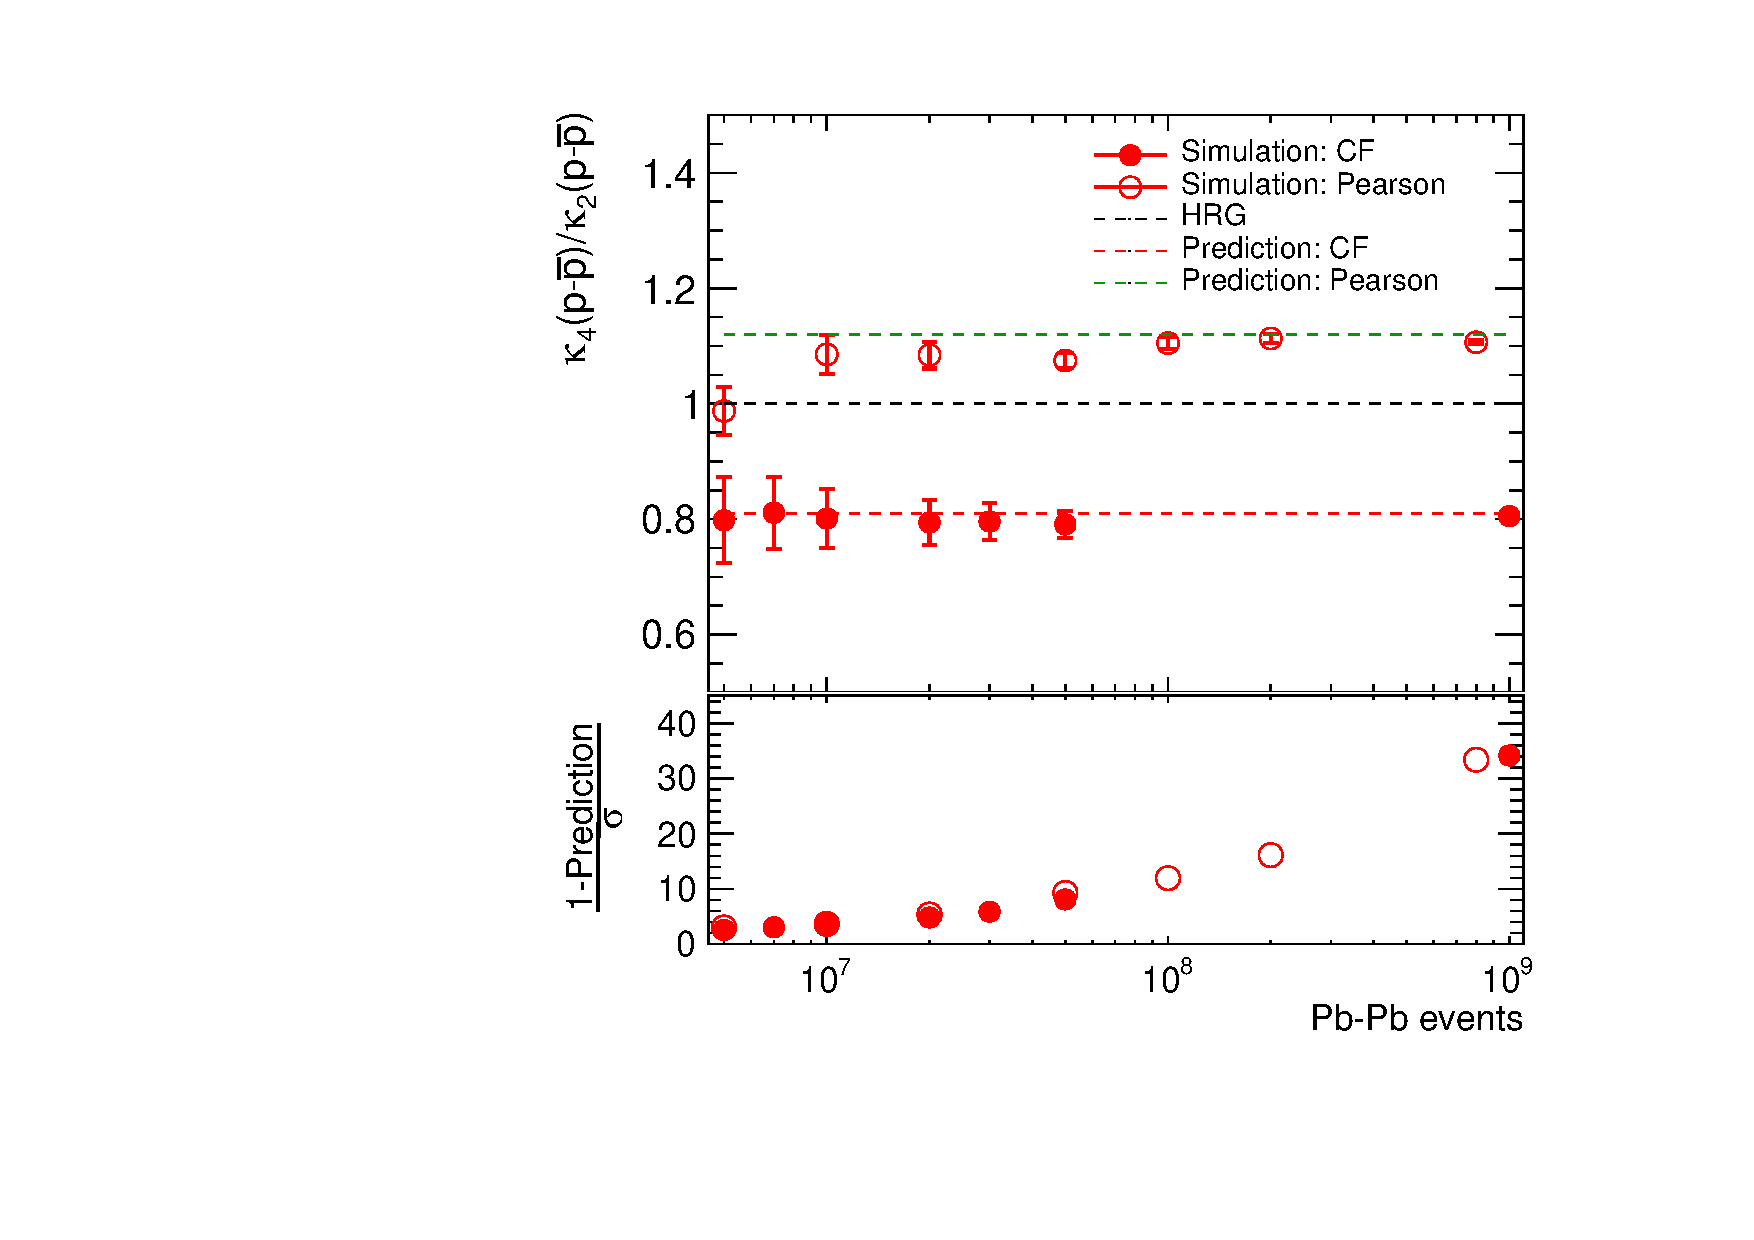
\includegraphics[width=0.45\textwidth]{\main/lightflavour/figs/stat42.pdf} &
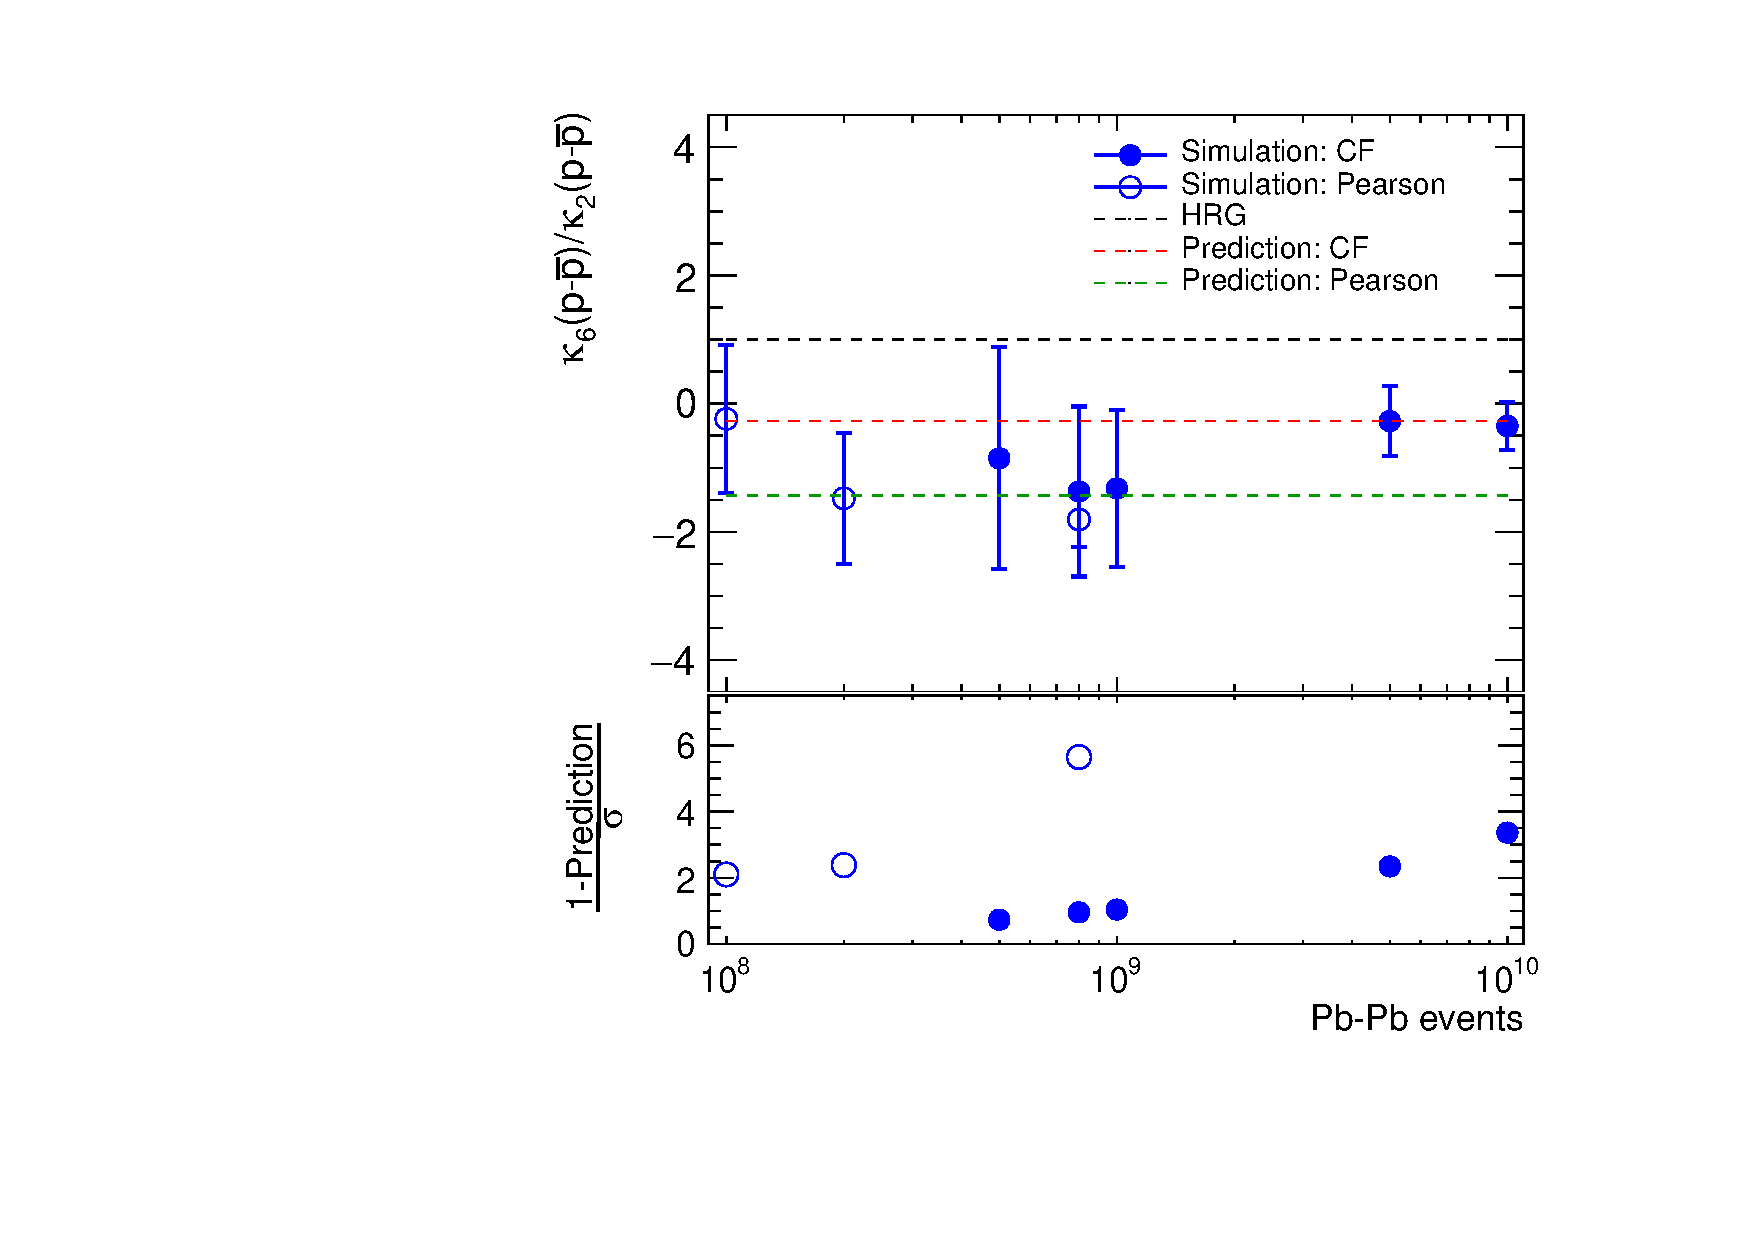
\includegraphics[width=0.45\textwidth]{\main/lightflavour/figs/stat62.pdf}
\end{array}$
\end{center}
\caption{Simulated values of  $\kappa_{4}/\kappa_{2}$ (left panel) and $\kappa_{6}/\kappa_{2}$ (right panel) as functions of the generated number of events. Full symbols represent results obtained with the double Gaussian approach adjusted to reproduce critical fluctuations (CF) predicted in the PQM model~\cite{Almasi:2017bhq}. Open symbols are obtained with the Pearson Curve Method\cite{Behera:2017xwg}.}
\label{fig:c4c2toymc}
\end{figure}




\clearpage
%%\subsection{Response functions}

% text from Stefan
%In a fluid dynamic description of heavy ion collisions,  one can understand the azimuthal harmonic flow coefficients $v_n$ as a response to deviations of the initial state from an isotropic form. Mathematically,  one can formulate this in terms of response functions that describe how the solution of the fluid dynamic evolution equations,  as well as resulting experimental observables such as azimuthal particle distributions,  get modified when the initial values of the fluid fields are changed. In cosmology,  closely related transfer functions are used to describe the response to initial density perturbations created by quantum fluctuations during inflation. Similar as in cosmology,  one can formulate linear as well as non-linear response functions for various fluid dynamic fields and observables. Moreover,  statistical symmetries of the initial state,  in particular azimuthal rotation invariance and the approximate Bjorken boost symmetry can be used to classify different perturbations. In the simplest implementation,  linear response functions describe the linear response of flow coefficients to eccentricities $v_n \sim\epsilon_n$,  while the quadratic part describes terms like $v_n \sim \epsilon_a\epsilon_b$ where symmetry reasons imply $|n|=|a\pm b|$. Response functions can not only be used to study deviations from azimuthal rotation symmetry but also for deviations from (approximate) Bjorken boost invariance,  vanishing baryon number density,  for electric fields and so on. Quite generally,  response functions cary interesting information about fluid properties such as thermodynamic and transport properties. Where the response functions are known,  one can infer properties of the initial state by reverse engineering.

%Experimentally,  one can constrain properties of response functions indirectly via measurements of various particle correlation functions. Differential information as well as good statistics are valuable here. It is particularly interesting to compare situations with strong deviations from a symmetry (such as peripheral collisions for the case of azimuthal rotation invariance) to situations with small deviations (such as central collisions). This should allow to distinguish linear from quadratic and higher order response functions.

%One may in principle also use classifications of events according to their net baryon number  in the central rapidity range or other event selection criteria. This idea is also known as event engineering and might become even more feasible with more statistics.

%A general problem in the context of the fluid dynamic description of heavy ion collisions is that the initial state is not very well known. For the time being,  one must improve the knowledge of the initial state as well as the fluid properties of the quark-gluon plasma (which in turn determine the response functions) simultaneously by detailed comparison between experimental results and theoretical calculations. Dependence on external parameters like system size and collision energy as well as differential information such as on centrality,   or particle identification will be helpful to make further progress here. In addition to this,  theoretical techniques and models must be improved further.




\subsection{Longitudinal flow fluctuations}

In nearly all traditional flow measurements the assumption is made that the 
  event-plane angles \psin\ do not change with $\eta$, i.e. that the \psin\
  are boost invariant.
This assumption is most clear in the event-plane and scalar-product methods
  of flow measurement,  where the \psin\ are measured at forward rapidities
  and the orientation of the reconstructed particles are then measured about
  these \psin~\cite{HION-2011-01,HION-2016-06}.
However multiple recent measurements at the LHC indicate the presence of 
  considerable longitudinal dynamics.
These include measurements from CMS of event-plane decorrelation in \ppb\ and \pbpb\ 
  collisions~\cite{CMS-HIN-14-012,CMS-HIN-15-008} and from ATLAS on flow-decorrelations~\cite{HION-2016-04}
  and forward-backward multiplicity fluctuations~\cite{HION-2015-13}.




\begin{figure*}[!htb]
\begin{center}
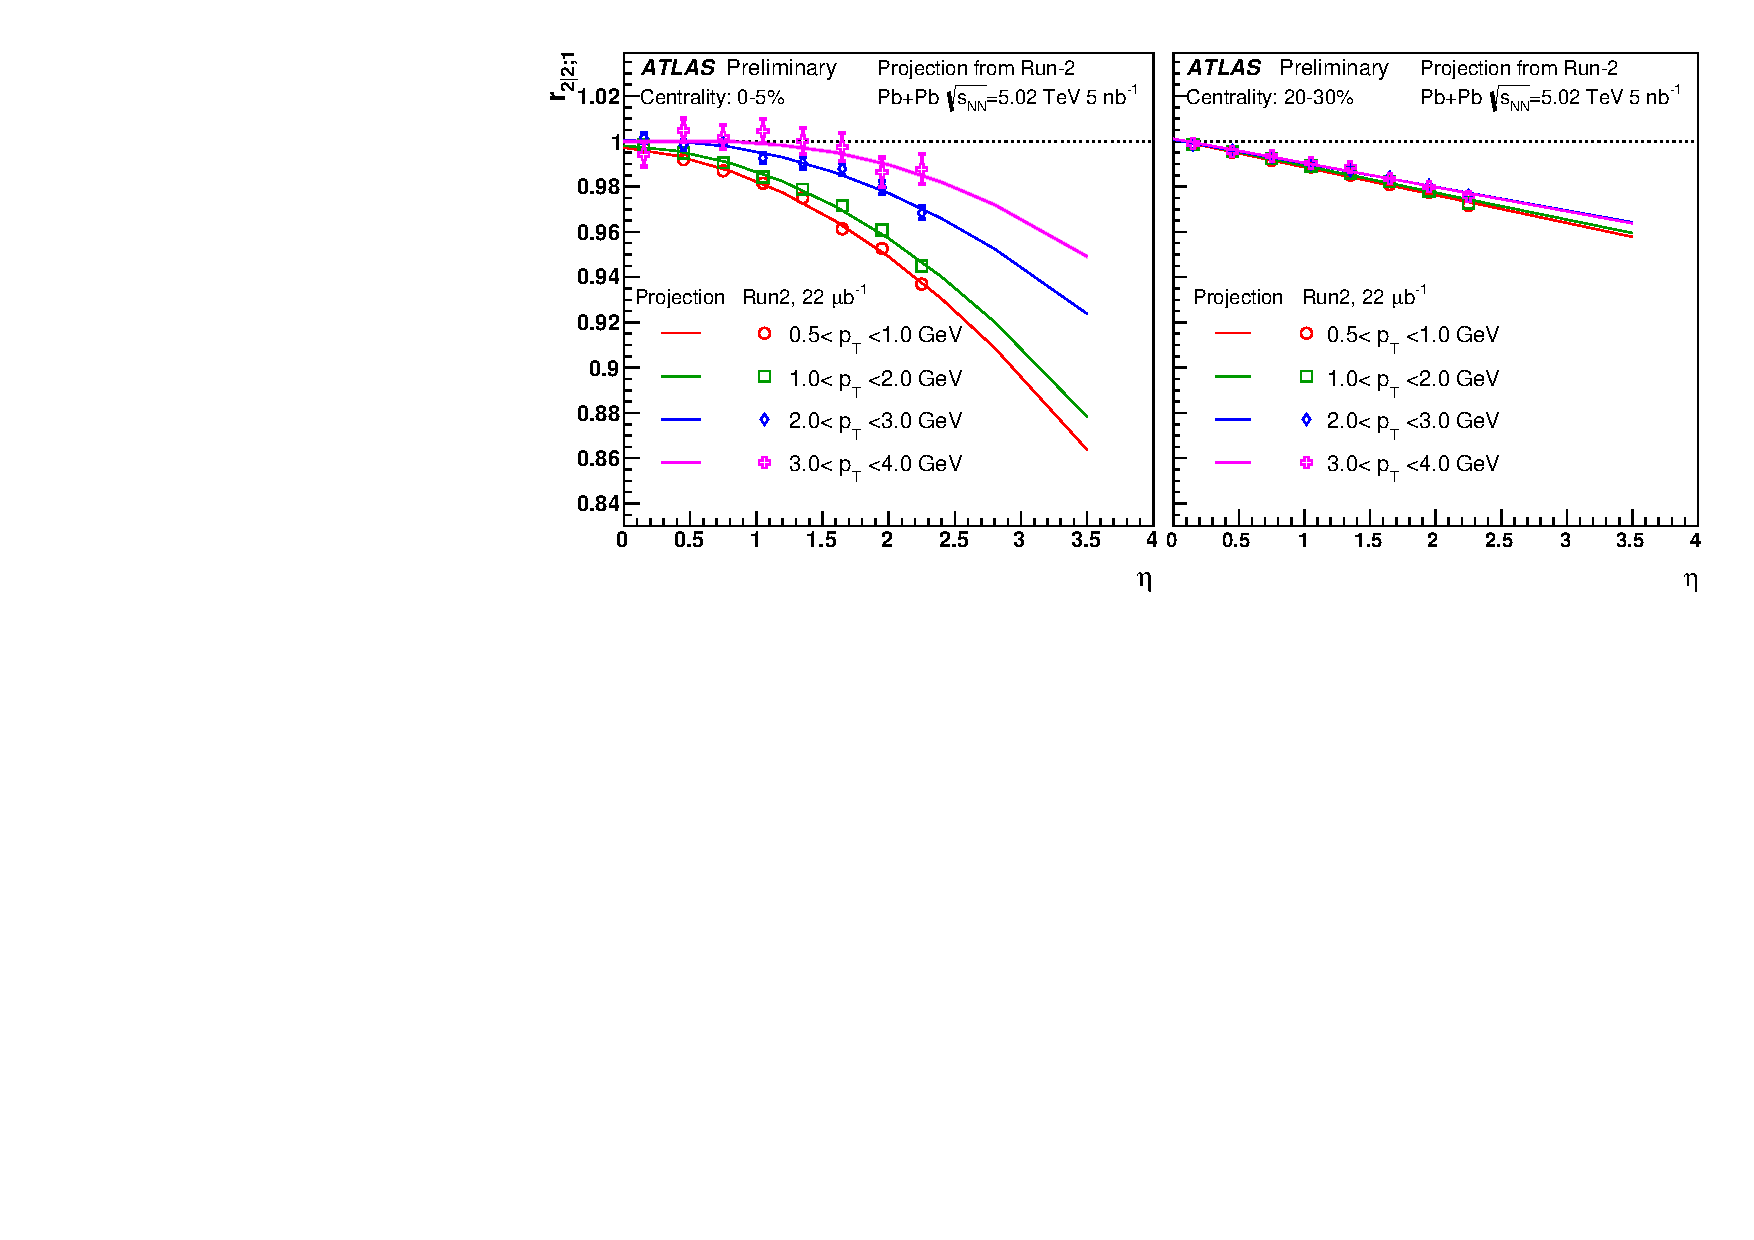
\includegraphics[width=0.8\textwidth]{\main/flow/figs/atlas_projection_r221}
\caption{
ATLAS projections of the flow-decorrelation observable $r_{2|2;1}$ 
  as a function of $\eta$ (lines).
The markers indicate the present measurements from Ref.~\cite{HION-2016-04}.
The left and right panels show projections for the 0--5\% and 20--30\%
  centrality intervals, respectively.
The width of the projection bands indicates the expected statistical uncertainty.
}
\label{fig:atlas_r221}
\end{center}
\end{figure*}


In the ATLAS measurements in Ref.~\cite{HION-2016-04}, the flow decorrelation 
  is quantified by constructing a correlator $r_{n|n;1}$ defined as:
\begin{equation}
r_{n|n;1}(\eta)=%
  \frac{\langle \mathbf{v}_n(-\eta)\mathbf{v}_n^*(\eta_{\mathrm{ref}})\rangle}%
  {\langle \mathbf{v}_n(\eta)\mathbf{v}_n^*(\eta_{\mathrm{ref}})\rangle},
\end{equation}
where $\mathbf{q}_n$ is the normalized flow vector, and $\eta_{\mathrm{ref}}$ is 
  the reference pseudo-rapidity~\cite{HION-2016-04}.
The correlator,  $r_{n|n;1}$,  measures the relative difference between flow
  $v_ne^{in\psin}$ at $\eta$ and $-\eta$.
If flow were boost-invariant, then $r_{n|n;1}$ would equal unity.
However any  difference in the $\eta$ dependence of the flow magnitude
  $v_n$ and the event plane angle \psin\ will lead to $r_{n|n;1}$
  become smaller than unity.
The present ATLAS measurements of $r_{2|2;1}$ over the 0--2.5 $\eta$ range 
  are shown in Figure~\ref{fig:atlas_r221} by the markers. 
It is observed that the $r_{2|2;1}$ is significantly smaller than unity 
  in central collisions, which indicates stronger flow decorrelation.
For a given centrality, $r_{2|2;1}$ decreases faster at low \pt\ 
  that at higher-\pt.
In the 20--30\% mid-central $r_{2|2;1}$ decreases linearly with $\eta$, 
  however in the 0--5\% most central collisions there are indications
  that the decorrelations are possibly quadratic.

Repeating this measurement in Run~4 will lead to significant improvements 
  due to increased luminosity and especially due to increased tracking 
  acceptance in $\eta$ to $\pm4$ units.
Figure~\ref{fig:atlas_r221} also shows the ATLAS projections for 
  $r_{2|2;1}$ made for Run~4, indicated as dashed lines.
The ATLAS tracking acceptance in Run~4 will extend the $\eta$ range 
  to $\pm$4 units, but the projected measurement is made
  to $\pm$3.5 units, in order to leave a gap between the ITk and the 
  region of the forward calorimeter in which the reference measurement 
  is made ($4.4<|\eta|<4.9$).
The projections are made by fitting the existing data with a linear 
  function for the 20--30\% centrality case and with a quadratic 
  function for the 0--5\% centrality case.
It is seen that with the increased $\eta$ acceptance the non-linearity 
  in the flow decorrelation can be studied in much more detail.


The longitudinal flow-decorrelation observables are sensitive to the 
  event by event fluctuations of the initial energy density profile 
  in the longitudinal direction. 
Thus precise measurement of these decorrelations should give
  a better understanding of the initial condition along the 
  longitudinal and in the development of full three-dimensional 
  viscous hydrodynamic models.
These would in turn result in a more accurate estimation of 
  $\eta/s$ from the model calculations.




%Soumya (+Wei)
\clearpage
\subsection{System size dependence}

\begin{itemize}
\item Motivation for colliding XeXe,  OO,  ArAr and other species
\item Analysis/measurement of deformation possible
\item disentangle geometry and viscous effects
\item interpolation points between Pb+Pb,  Cu+Cu,  p/D/He+A
\end{itemize}


\begin{figure}[!htb]
\begin{center}
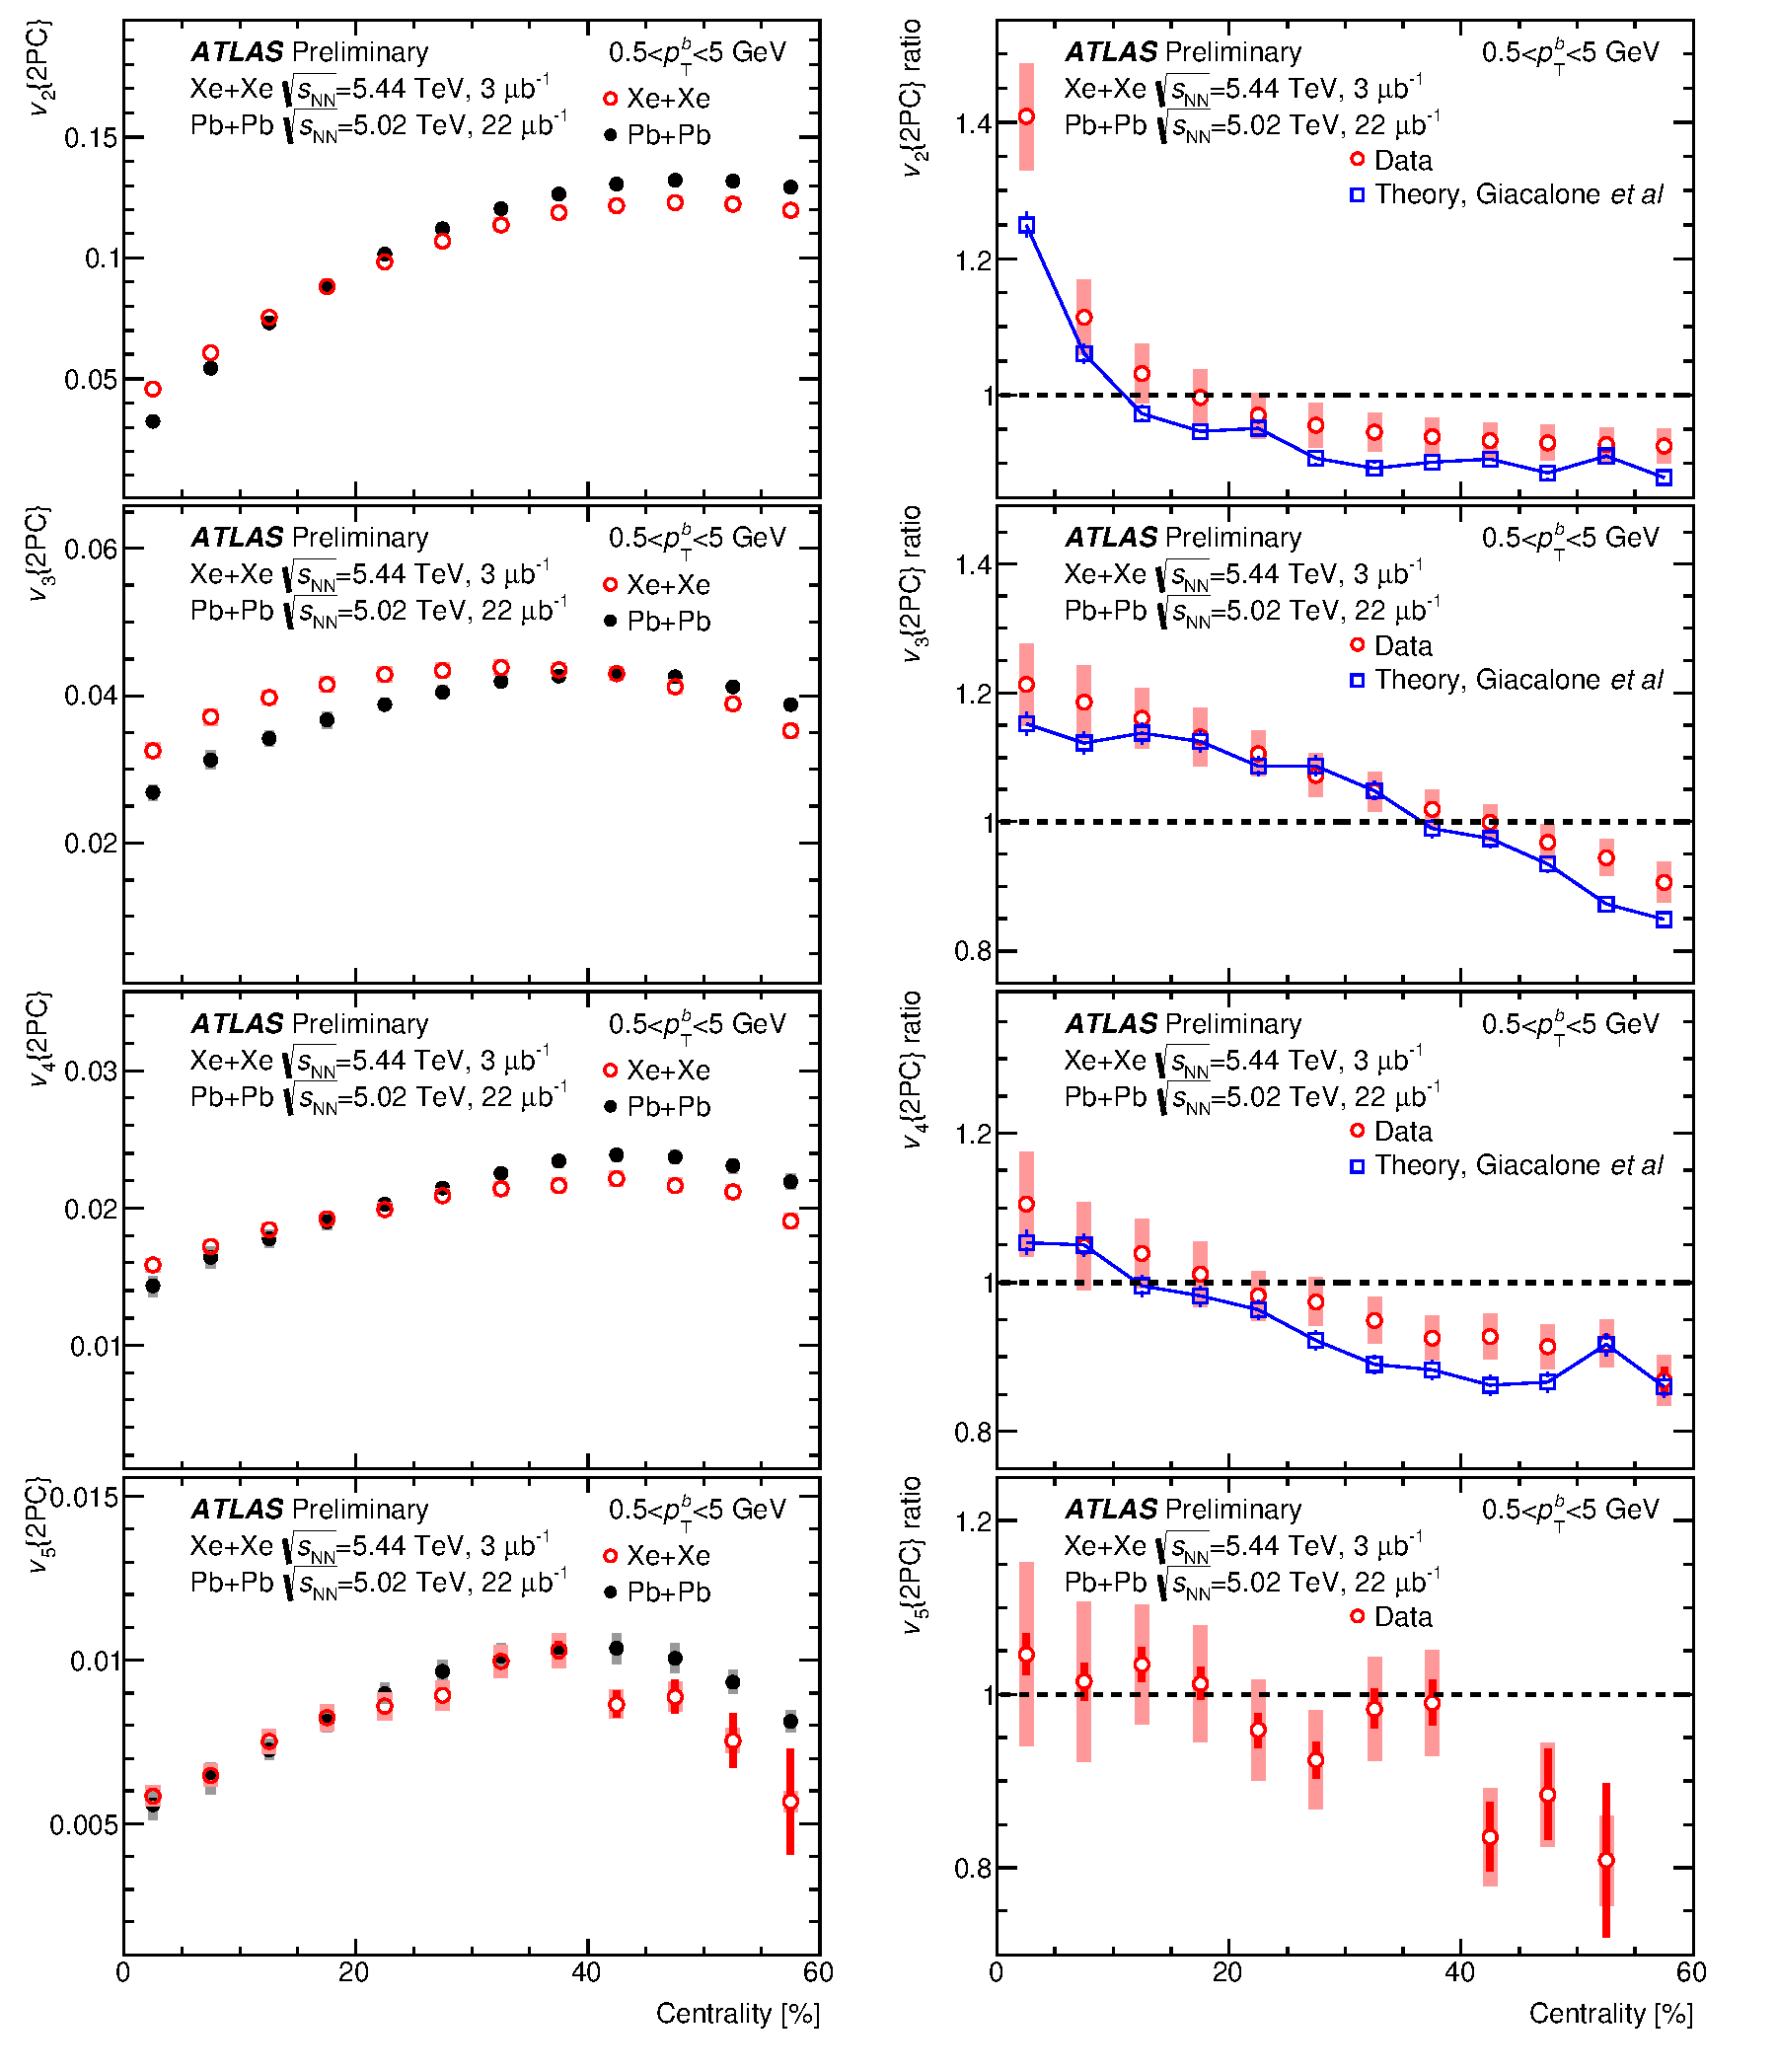
\includegraphics[width=0.8\textwidth]{figs/atlas_xexe_vn}
\caption{
	Figure from Ref.~\cite{ATLAS-CONF-2018-011}
}
\label{fig:atlas_xexe_vn}
\end{center}
\end{figure}
%Bjoern
\clearpage
\subsection{Vorticity and polarization}

An interesting open question for relativistic fluids is to what extend the spin degrees of freedom thermalize locally and to what extend spin polarization results as a consequence of the fluid motion. Intuitively, one might expect that spin aligns locally with the rotational motion of the fluid as measured by vorticity, corresponding to the curl of the fluid velocity.

The relativistic generalization of the non-relativistic fluid vorticity is non unambiguous, however. The vorticity of a fluid in local equilibrium is characterized by the so-called thermal vorticity tensor, corresponding to $\omega_{\mu\nu} = \frac{1}{2} (\nabla_\nu \beta_\mu - \nabla_\mu \beta_\nu)$ where $\beta_\mu=u_\mu / T$ is the ratio of fluid velocity to temerature \cite{Becattini:2013fla}. This thermal vorticity has then contributions from rotational motion, local fluid acceleration, and temperature gradients. It has been argued, that local spin polarization should follow this thermal vorticity. If this holds at chemical freeze-out, one should be able to find traces of the thermal vorticity in the polarization of particles and resonances with spin, such as Lambda and (anti-) Lambda resonances.

Spin polarization is in this picture closely tied to angular momentum of the expanding fireball. For non-central events, an angular momentum of the produced matter can result that points into the transverse plane, orthogonal to the event plane. Via the spin-vorticity coupling mechanism, this leads to global polarization in the transverse plane (along global angular momentum) which has recently also been found experimentally at RHIC [citations]. For this global effect following global angular momentum, one expects a decreasing magnitude with increasing collision energy and the effect is expected to be relatively small at LHC energies. 

In addition to that, there is also the expectation of a azimuthally dependent, longitudinal polarization (in the direction of the beam pipe). This is mainly a consequence of an azimuthal dependence of local acceleration and temperature gradient and should lead for non-central collisions mainly to an elliptic modulation of spin polarization. This effect has a weaker dependence on collision energy and should be almost as large at the LHC as at RHIC \cite{Karpenko:2017dui}. It would be highly interesting to investigate polarization effects of Lambdas and other resonances in more detail at the LHC and to map out the dependence on azimuthal angle, rapidity, transverse momentum etc.




\begin{itemize}
	\item
The estimation for the LHC energy $\sqrt{s_{NN}}=2.76$ TeV indicate the strength of Abelian magnetic field is $eB \sim 1.0$ GeV$^{2}$ very shortly after collisions and it decreases down to the $eB \sim 200$ MeV$^{2}$ for time $\tau \sim 0.1$ fm/$c$ without taken into account the electroconductivity of the quark-gluon matter \cite{AHEP-2014-193039-2014,JPCS-668-012129-2016,JPCS-675-022021-2016}. Therefore one can expect $|\Delta P|=0.61eB/m_{p}T \sim (4.3 \pm 0.7) \times 10^{-4}$ for the temperature of the quark-gluon plasma $T=(304 \pm 51)$ MeV \cite{NPA-904-905-573c-2013}. Here $m_{p}$ is the proton mass, $\Delta P \equiv P_{\Lambda}-P_{\bar{\Lambda}}$ is the difference in polarization of primary $\Lambda$ and $\bar{\Lambda}$ \cite{PRC-95-054902-2017}. This estimation for $|\Delta P|$ is some smaller than that at RHIC energies due to hotter medium at the LHC. But it should be noted the electroconductivity will lead to noticeably weaker time dependence of the $eB$ \cite{AHEP-2013-490495-2013} and the conductivity may compensate the growth of $T$ and provides the increase of the $|\Delta P|$. Moreover the pass from RHIC to the LHC energy leads to the significant growth of the peak value for $eB$. Thus for HE--LHC the magnitude of $\Delta P$ is expected similar or even larger than at RHIC energies. Furthermore the higher energy of the HE--LHC project provides the novel opportunity for study of polarization of heavier hyperons (for instance, $\Sigma$) in hot environment.
\end{itemize}

\begin{figure}[!htb]
\begin{center}
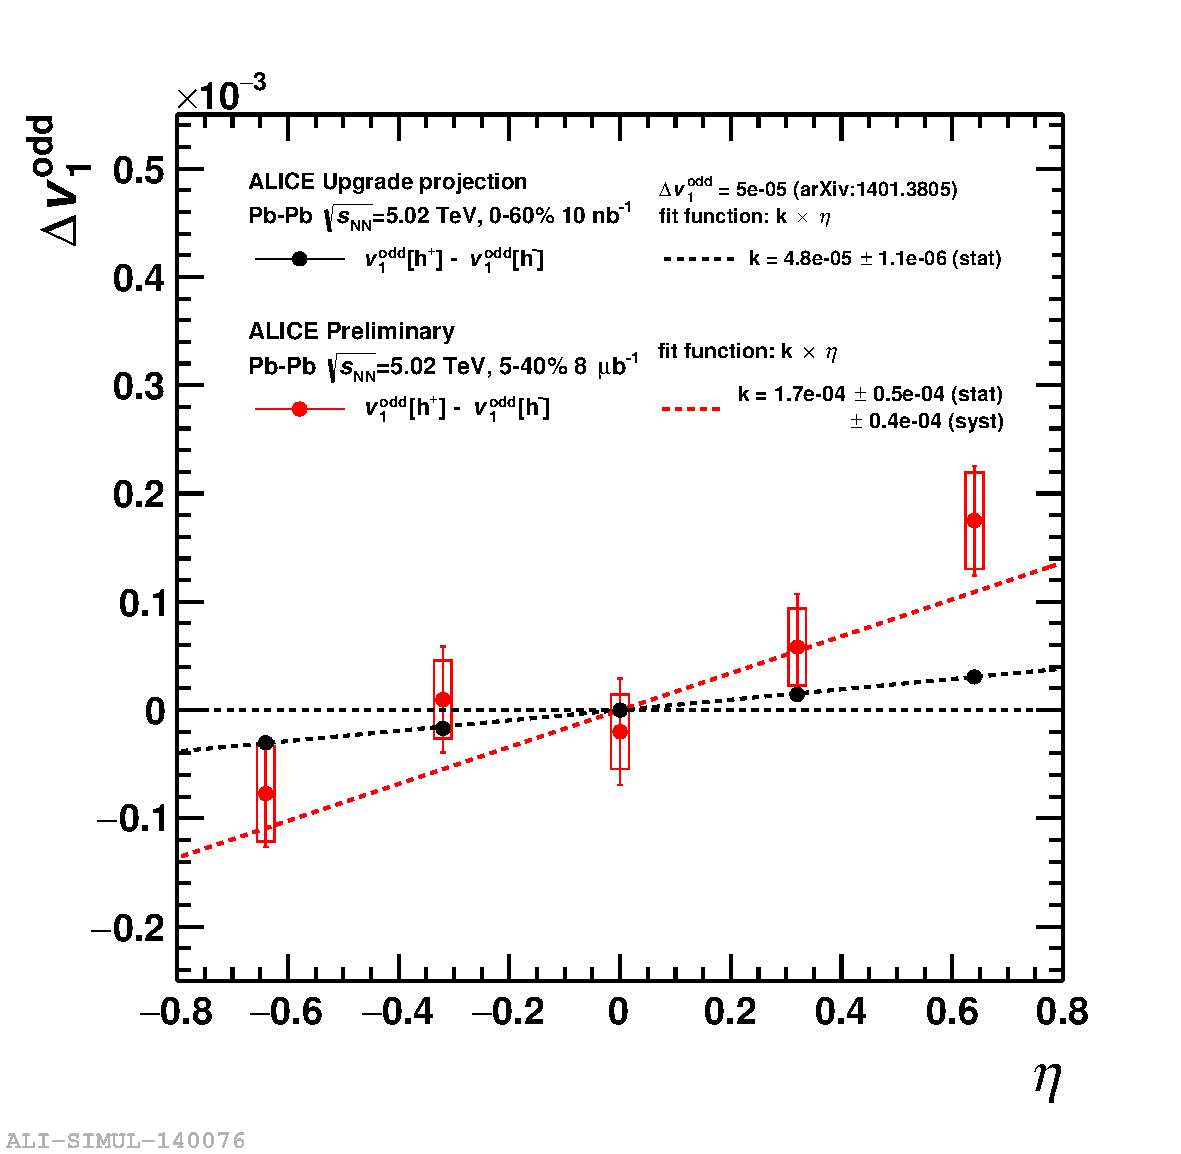
\includegraphics[width=0.8\textwidth]{\main/flow/figs/alice_projection_deltav1ch_stat8}
\caption{
}
\label{fig:alice_delta_v1}
\end{center}
\end{figure}


\begin{figure*}[!htb]
\begin{center}
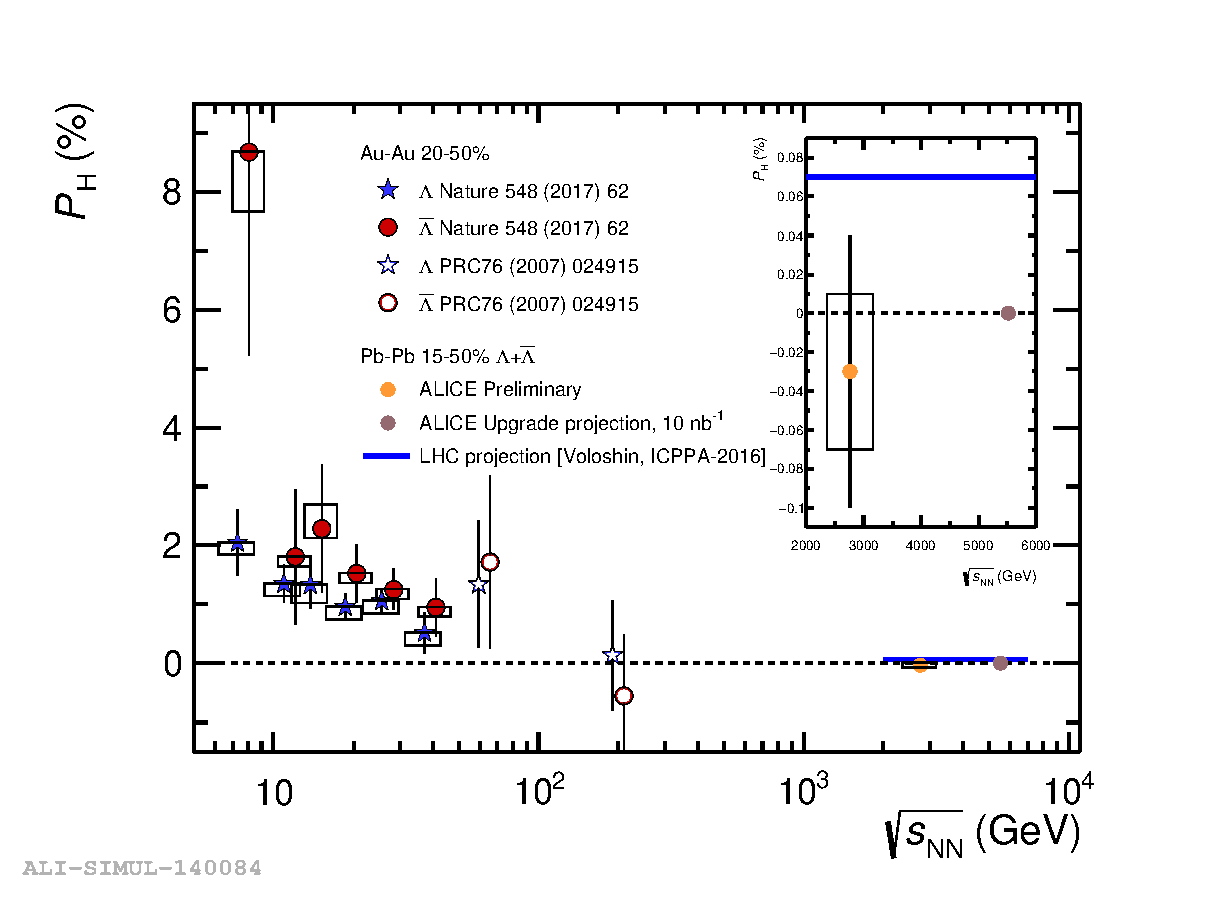
\includegraphics[width=0.8\textwidth]{\main/flow/figs/alice_projection_lambda}
\caption{Global polarization of $\Lambda$ and $\bar{\Lambda}$ as a function of the collision energy $\sqrt{s_{NN}}$ for semi-central heavy ion collisions. Open boxes
and vertical lines show systematic and statistical uncertainties,
respectively. Main panel: the data points for $\bar{\Lambda}$ are slightly horizontally shifted for visibility. Inner panel: the LHC energy domain is shown more detailed.
}
\label{fig:alice_lambda}
\end{center}
\end{figure*}

Fig. \ref{fig:alice_lambda} presents the energy dependence of the global polarization of $\Lambda$ and $\bar{\Lambda}$ for the semi-central heavy ion collisions. The RHIC results show the decrease of polarization at higher $\sqrt{s_{NN}}$. But $\Lambda$ and $\bar{\Lambda}$ demonstrate the finite global polarizations even at highest RHIC energy $\sqrt{s_{NN}}=200$ GeV \cite{PRC-98-014910-2018}. The preliminary ALICE data point at $\sqrt{s_{NN}}=2.76$ TeV is close in magnitude with results at $\sqrt{s_{NN}}=200$ GeV. But the ALICE upgrade projection at twice large collision energy corresponds to the zero polarization with very high precision. Therefore the study of global polarization of $\Lambda$ and $\bar{\Lambda}$ within HL--LHC project allows the unambiguous conclusion with regard of the values of this physics quantity in TeV-energy domain.    
%Stefan,Alex
\clearpage
\subsection{Chiral Magnetic Effect}

%\begin{itemize}
%	\item
%The vacuum of quantum chromodynamics (QCD) is characterized by rich geometry structure which may corresponds to the fractal-like geometry \cite{IJMPE-22-1350041-2013}.There is a fundamental interrelation between geometry and essential properties of QCD Lagrangian.Structures with non-trivial topology in QCD vacuum are believed to determine the behavior of the $\mathcal{P / CP}$ fundamental symmetries in the hot quark-gluon matter. Due to higher luminosity at the HL--LHC and / or high multiplicity per event at HE--LHC energy the multiparticle azimuthal correlations can be used for investigations of wide set of chiral effects in strong interaction \cite{PAN-80-1133-2017}, for instance, chiral magnetic effect -- CME, chiral magnetic waves -- CMW etc. This approach  allows the significant suppression of the backgrounds and improvement of reliability of physical conclusions. The study of charge-dependent azimuthal correlations for various types of light flavor particles can be possible with unprecedented precision due to high luminosity of the HL--LHC project. Consequently the quantitative comparison will be allowed for strengths of correlations in meson, baryon--meson and baryon systems. Such measurements will be essential in particular for search for chiral vortical effect -- CVE and its study with high precision. Furthermore the higher energies of the HE--LHC project can provide the opportunity for study of flavor dependence of the $\mathcal{P / CP}$ violation with help the azimuthal correlations for wider set of types of secondary particles including for heavy flavor ones. Thus experimental study of topology of QCD vacuum can be one of the focuses for studies of bulk properties within the HL--LHC, HE--LHC projects.
%\end{itemize}

An important property of the strong interaction which is potentially observable in heavy-ion collisions is parity violation. Although it is allowed by 
quantum chromodynamics (QCD), global parity violation is not observed in strong interaction. However, QCD predicts the existence of topologically 
non-trivial configurations of the gluonic field, instantons and sphalerons, which might be responsible for local parity violation in microscopic QCD 
domains at finite temperature \cite{Lee:1973iz, Lee:1974ma, Morley:1983wr, Kharzeev:1998kz}. The $P$- and $CP$-odd interactions between quarks 
and such fields with non-zero topological charge~\cite{Chern:1974ft} change the quark chirality, breaking parity symmetry by creating an imbalance 
between the number of left- and right-handed quarks. Furthermore, an extremely strong magnetic field is expected to be produced in heavy-ion collisions 
\cite{Deng:2012pc, Gursoy:2014aka} (of the order of $10^{19}$ Gauss at the LHC) because the charges of initial ions add coherently. This strong 
magnetic field aligns the spins of the negatively (positively) charged quarks in the direction anti-parallel (parallel) to magnetic field orientation. Moreover, 
right-handed (left-handed) quarks have their direction of momentum parallel (anti-parallel) to the spin orientation. The spin alignment coupled with the 
local imbalance between the number of left- and right-handed quarks leads to the development of a quark current. The current moves the positively 
charged quarks along its direction and the negatively charged quarks in the opposite direction. This implies a charge separation along the direction 
of the magnetic field, which is on average perpendicular to the symmetry plane (defined by the participant nucleons and the beam direction), a 
phenomenon called Chiral Magnetic Effect (CME) \cite{Kharzeev:2004ey, Kharzeev:2007tn, Kharzeev:2007jp, Fukushima:2008xe}. 

Since the sign of 
the topological charge is equally probable to give rise to a positive or negative current in the magnetic field direction, the charge separation averaged 
over many events is zero. This makes the observation of the CME experimentally difficult and possible only via azimuthal particle correlations, which 
introduces a large flow related background into the measurements.

The three-particle correlator $\gamma_{\alpha\beta} = \langle \cos(\varphi_{\alpha} + \varphi_{\beta} - 2\Psi_{\rm 2}) \rangle$ \cite{Voloshin:2004vk}, 
where $\varphi_{\alpha}$ is the azimuthal angle of the particle of charge $\alpha$ and $\Psi_{\rm 2}$ is the second harmonic symmetry plane 
angle, was proposed to measure charge-dependent azimuthal correlations. This correlator eliminates correlations independent of symmetry 
plane orientation, suppressing background contributions at the level of $\sim v_2$. However, the interpretation of the experimental results is 
complicated by the remaining background (e.g. local charge conservation (LCC) coupled with elliptic flow~\cite{Schlichting:2010qia, Pratt:2010zn}). 
Recent observation of similar charge-dependent azimuthal correlations in pPb (where the CME is not expected) and 
PbPb collisions~\cite{Khachatryan:2016got} indicates 
the $\gamma_{\alpha\beta}$ correlator be dominated, if not all, by the background effect.
The ALICE \cite{Acharya:2017fau} and CMS \cite{Sirunyan:2017quh} collaborations have used the Event Shape Engineering (ESE) technique 
\cite{Schukraft:2012ah} to estimate the CME fraction to the charge dependence of $\gamma_{\alpha\beta}$, $f_{\rm CME}$, in PbPb collisions. 
ALICE extracted 
$f_{\rm CME}$ by relating measurements of the charge dependence of $\gamma_{\alpha\beta}$ from the ESE analysis to CME signal expectations from 
various initial state model calculations including a magnetic field. It has been assumed that the CME signal is proportional to 
$\langle |B|^2 \cos(2(\Psi_{\rm B} - \Psi_2)) \rangle$, where $|B|$ and $\Psi_{\rm B}$ are the magnitude and direction of the magnetic field, respectively. Within current experimental uncertainties, the CME signal contribution to the $\gamma_{\alpha\beta}$ correlator is consistent with zero.

Figure~\ref{fig:alice_fcme} shows the upper limit on $f_{\rm CME}$ at 95\% confidence level for the 20--30\% centrality interval reported by the 
ALICE collaboration together with expectations for $f_{\rm CME}=0.164$ and $f_{\rm CME}=0$ as a function of the number of events. The shaded 
boxes denote variations due to different estimates of the magnetic field from the investigated models. The ALICE upgrade projection indicates that 
stringent constraints for the CME contribution to the charge dependence of $\gamma_{\alpha\beta}$ can be achieved to a level of less than 1\% 
with the expected HL--LHC statistics. 

\begin{figure}[!htb]
\begin{center}
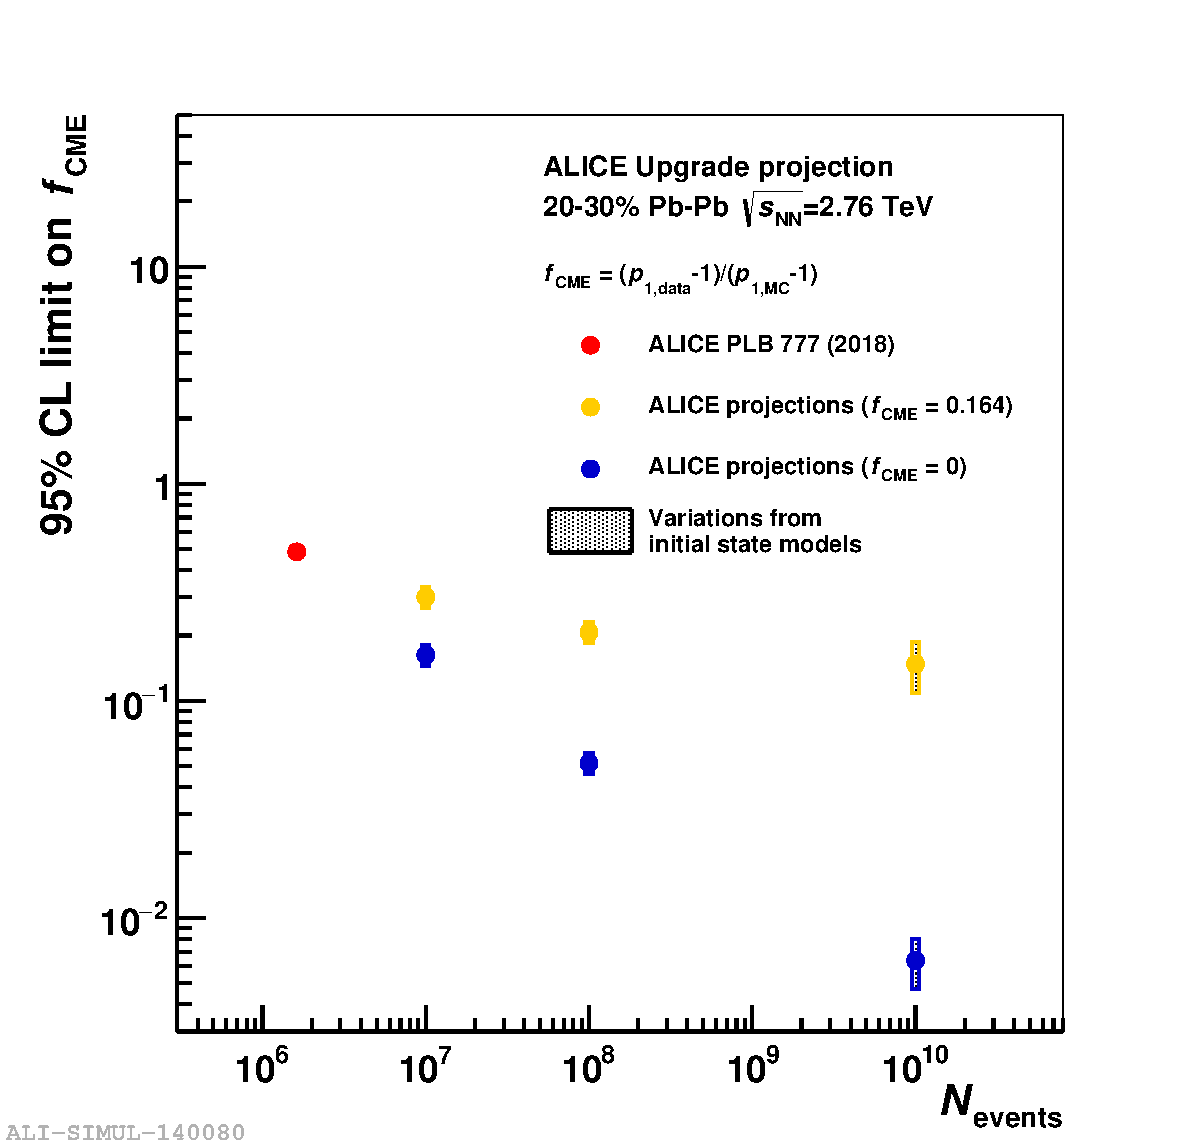
\includegraphics[width=0.8\textwidth]{\main/flow/figs/alice_projection_fcme}
\caption{The upper limit on the CME fraction at 95\% confidence level as a function of the number of events in the 20--30\% centrality interval. The result reported by the ALICE collaboration \cite{Acharya:2017fau} is shown together with expectations for $f_{\rm CME}=0.164$ and $f_{\rm CME}=0$. The shaded boxes denote variations from various initial state models (see text for details).}
\label{fig:alice_fcme}
\end{center}
\end{figure}

One key ingredient needed for the observation of the CME is the strong magnetic field in the QGP medium. It is important to establish a direct
evidence for the presence of this field on final-state particles and to calibrate its strength, which will help significantly constrain theoretical predictions on the magnitude of the CME signal. Measurement of the pseudorapidity-odd component of directed 
flow, $v_1^{\rm odd}$, separately for positive and negative charged particles has been proposed as a probe to 
the magnetic field~\cite{Gursoy:2014aka}. Any difference will indicate the presence of induced electromagnetic 
currents and will allow to estimate the magnitude of the effect. It will also provide information on the electric conductivity of the QGP medium.


\begin{figure}[!htb]
\begin{center}
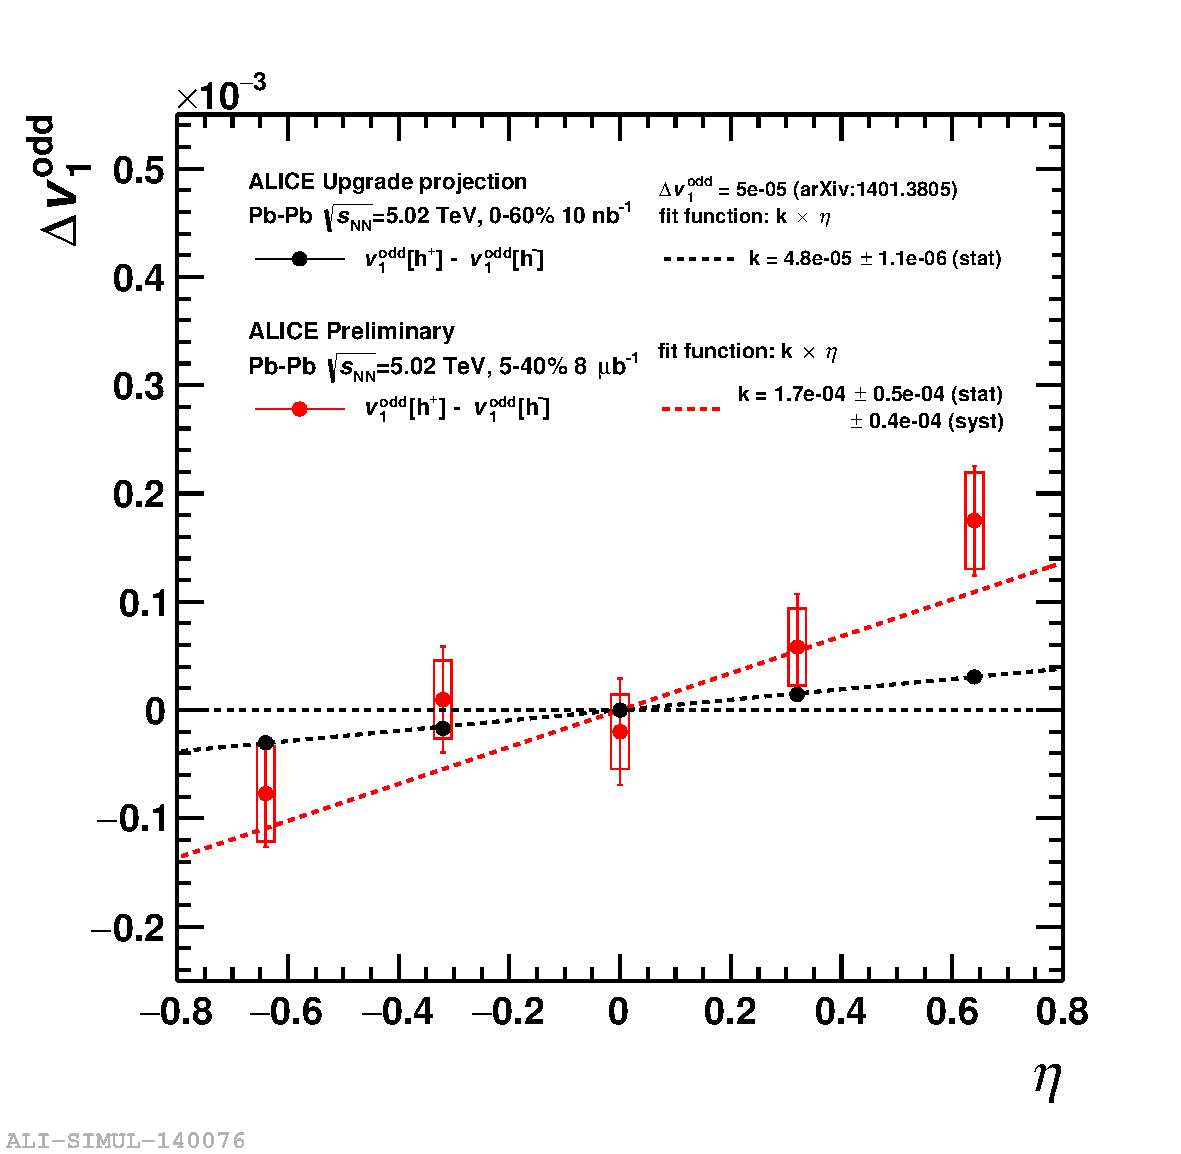
\includegraphics[width=0.8\textwidth]{\main/flow/figs/alice_projection_deltav1ch_stat8}
\caption{Charge difference of $v_1^{\rm odd}$ as a function of pseudorapidity measured by the ALICE collaboration in Pb--Pb collisions at $\sqrt{s_{NN}}=5.02$ TeV  \cite{Margutti:2017lup} (red symbols) and the expectation for a $5 \times 10^{-5}$ difference \cite{Gursoy:2014aka} from 10 nb$^{-1}$ (black symbols) together with linear fits (dashed lines). Error bars (open boxes) represent the statistical (systematic) uncertainties.}
\label{fig:alice_delta_v1}
\end{center}
\end{figure}


Figure~\ref{fig:alice_delta_v1} shows the charge difference of $v_1^{\rm odd}$, 
$\Delta v_1^{\rm odd}=v_1^{\rm odd +} - v_1^{\rm odd -}$, as a function of pseudorapidity measured by the ALICE collaboration in Pb--Pb collisions 
at $\sqrt{s_{NN}}=5.02$ TeV \cite{Margutti:2017lup} together with a linear fit. A hint of a charge-dependent difference is observed and quantified 
by the slope $k$ with a total significance of 2.6 $\sigma$. This difference, which differs both in magnitude and sign compared to predictions for 
$\pi^{\pm}$ at $\sqrt{s_{NN}}=2.76$ TeV and similar $\langle p_{\rm T} \rangle$ \cite{Gursoy:2014aka}, needs to be confirmed. 
This will be achieved 
with the large data sample expected at the HL--LHC where even the predicted difference of $5 \times 10^{-5}$ will be measured with high accuracy 
as reported by the ALICE upgrade projection in Fig. \ref{fig:alice_delta_v1}. Furthermore, similar measurement can also be performed
in the heavy flavor sector, e.g., for $D^{0}$ and $\bar{D^{0}}$ meson directed flow~\cite{Das:2016cwd}. Heavy flavor quarks have the advantage of
being produced at a very early stage, and thus potentially have a better sensitivity to the magnetic field at its peak magnitude before it decays.




 %Wei, Vitaly
\clearpage
\subsection{Summary}
The measurements of inclusive hadron \vn\ by traditional methods such as 
  two-particle correlations, event-plane/scalar-product methods, 
  multi-particle cumulants etc. have been performed with high precision 
  by the ALICE, ATLAS and CMS experiments at the LHC.
These inclusive hadron \vn\ measurements are not statistically limited 
  across most of the centrality-\pt\ phase space and further improvement 
  in the measurements is not a high priority for Run~3 and 4.
However, in the case of identified hadrons the increased statistics 
  will lead to further improvement in the \vn\ measurements.
This is true for both light hadrons such as pions, protons, $\phi$-mesons 
  as shown in Figure~\ref{fig:alice_vn}, as well as for heavy-flavor 
  particles such as $D^0$, $D^{\pm}$, J/$\psi$, $\Upsilon$ which are 
  discussed in Chapters~\ref{sec:HI_HF} and \ref{sec:quarkonia}, respectively.
%
Significant improvements are expected in measurements of 
  longitudinal flow fluctuations, which have only been briefly investigated
  in Run~1 and 2.
These are largely driven by the increases $\eta$ acceptance of the
  ATLAS and CMS tracking detectors in Run~4, the acceptance is planned 
  to reach $\pm$5 units.
The study of longitudinal flow fluctuations will allow comparisons to predictions 
  of 3+1D hydro models.
%
Flow measurements in light ions such as Ar--Ar and O--O, will lead 
  to stronger constraints on theoretical models describing different 
  stages of a heavy ion collision 
  -- initial conditions, equation of state, transport coefficients etc.
This is difficult presently, as flow observables are simultaneously dependent 
  on all of these, so it becomes difficult to constrain one any one of these 
  without full knowledge of the others.
Flow measurements across a variety of colliding species will provide independent 
  data points that can help in improvement of our understanding of these different 
  stages of heavy ion collisions.
Further physics motivations for colliding light are discussed in Chapter~\ref{sec:smallAsum}.

Other observables related to collective phenomena where current 
  measurements are statistics limited and are expected to improve 
  considerably are related to effects of vorticity and magnetic fields.
%
The current measurements of $\Lambda$ polarization from ALICE are statistics limited
  and consistent with both the null hypothesis as well as with the theoretically
  predicated value.
The ALICE projections for $\Lambda$ polarization in Run~3 and 4 show that 
  the measurements will have significantly smaller statistical uncertainties 
  and will easily be able to differentiate between the null and predicted values. 
%
ALICE and CMS have measured the fraction of the three-particle correlator
  $\gamma_{\alpha\beta}$ that arises from CME effects: $f_{\mathrm{CME}}$.
The measured $f_{\mathrm{CME}}$ by ALICE is consistent with zero but due to 
  large uncertainties its upper limit at 95\% CL can be as large as $\sim$0.5.
ALICE projections for Run~3 and 4 show that the $f_{\mathrm{CME}}$ can 
  be determined with a precision of less than 1\%.


















 %Soumya, Wei

\end{document}

